% Created by tikzDevice version 0.12.3 on 2020-02-03 16:01:28
% !TEX encoding = UTF-8 Unicode
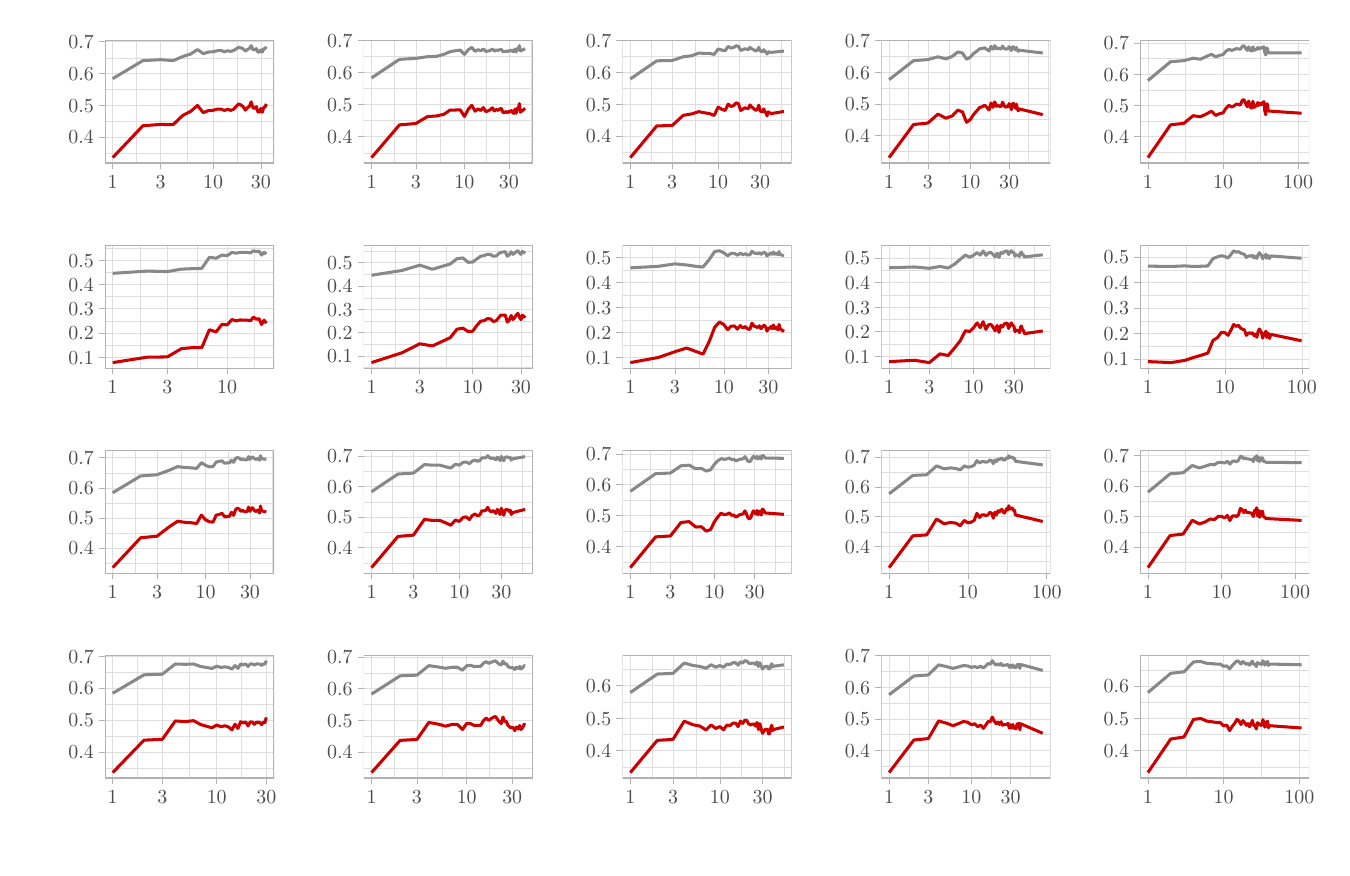
\begin{tikzpicture}[x=1pt,y=1pt]
\definecolor{fillColor}{RGB}{255,255,255}
\path[use as bounding box,fill=fillColor,fill opacity=0.00] (0,0) rectangle (467.59,296.31);
\begin{scope}
\path[clip] (  0.00,222.23) rectangle ( 93.52,296.31);
\definecolor{drawColor}{RGB}{255,255,255}
\definecolor{fillColor}{RGB}{255,255,255}

\path[draw=drawColor,line width= 0.5pt,line join=round,line cap=round,fill=fillColor] (  0.00,222.23) rectangle ( 93.52,296.31);
\end{scope}
\begin{scope}
\path[clip] ( 27.95,247.34) rectangle ( 89.02,291.81);
\definecolor{fillColor}{RGB}{255,255,255}

\path[fill=fillColor] ( 27.95,247.34) rectangle ( 89.02,291.81);
\definecolor{drawColor}{gray}{0.87}

\path[draw=drawColor,line width= 0.1pt,line join=round] ( 27.95,251.06) --
	( 89.02,251.06);

\path[draw=drawColor,line width= 0.1pt,line join=round] ( 27.95,262.53) --
	( 89.02,262.53);

\path[draw=drawColor,line width= 0.1pt,line join=round] ( 27.95,274.00) --
	( 89.02,274.00);

\path[draw=drawColor,line width= 0.1pt,line join=round] ( 27.95,285.47) --
	( 89.02,285.47);

\path[draw=drawColor,line width= 0.1pt,line join=round] ( 39.37,247.34) --
	( 39.37,291.81);

\path[draw=drawColor,line width= 0.1pt,line join=round] ( 57.50,247.34) --
	( 57.50,291.81);

\path[draw=drawColor,line width= 0.1pt,line join=round] ( 75.62,247.34) --
	( 75.62,291.81);

\path[draw=drawColor,line width= 0.2pt,line join=round] ( 27.95,256.79) --
	( 89.02,256.79);

\path[draw=drawColor,line width= 0.2pt,line join=round] ( 27.95,268.27) --
	( 89.02,268.27);

\path[draw=drawColor,line width= 0.2pt,line join=round] ( 27.95,279.74) --
	( 89.02,279.74);

\path[draw=drawColor,line width= 0.2pt,line join=round] ( 27.95,291.21) --
	( 89.02,291.21);

\path[draw=drawColor,line width= 0.2pt,line join=round] ( 30.72,247.34) --
	( 30.72,291.81);

\path[draw=drawColor,line width= 0.2pt,line join=round] ( 48.02,247.34) --
	( 48.02,291.81);

\path[draw=drawColor,line width= 0.2pt,line join=round] ( 66.97,247.34) --
	( 66.97,291.81);

\path[draw=drawColor,line width= 0.2pt,line join=round] ( 84.27,247.34) --
	( 84.27,291.81);
\definecolor{drawColor}{RGB}{136,136,136}

\path[draw=drawColor,line width= 1.1pt,line join=round] ( 30.72,277.87) --
	( 41.63,284.40) --
	( 48.02,284.74) --
	( 52.55,284.40) --
	( 56.06,285.89) --
	( 58.93,286.80) --
	( 61.36,288.41) --
	( 63.46,286.92) --
	( 65.32,287.50) --
	( 66.97,287.61) --
	( 68.47,287.96) --
	( 69.84,288.07) --
	( 71.10,287.61) --
	( 72.27,287.96) --
	( 73.36,287.72) --
	( 74.37,288.05) --
	( 75.33,288.63) --
	( 76.23,289.21) --
	( 77.08,288.98) --
	( 77.89,288.64) --
	( 78.66,287.84) --
	( 79.39,288.41) --
	( 80.09,288.75) --
	( 80.76,289.79) --
	( 81.40,288.40) --
	( 82.02,288.30) --
	( 82.61,288.76) --
	( 83.18,287.51) --
	( 83.74,287.50) --
	( 84.27,288.30) --
	( 84.79,287.50) --
	( 85.29,288.64) --
	( 85.77,288.76) --
	( 86.24,289.44);
\definecolor{drawColor}{RGB}{204,0,0}

\path[draw=drawColor,line width= 1.1pt,line join=round] ( 30.72,249.36) --
	( 41.63,260.86) --
	( 48.02,261.35) --
	( 52.55,261.25) --
	( 56.06,264.62) --
	( 58.93,266.09) --
	( 61.36,268.21) --
	( 63.46,265.59) --
	( 65.32,266.35) --
	( 66.97,266.44) --
	( 68.47,266.89) --
	( 69.84,266.86) --
	( 71.10,266.42) --
	( 72.27,266.81) --
	( 73.36,266.43) --
	( 74.37,266.80) --
	( 75.33,267.82) --
	( 76.23,268.75) --
	( 77.08,268.35) --
	( 77.89,267.74) --
	( 78.66,266.51) --
	( 79.39,267.34) --
	( 80.09,267.84) --
	( 80.76,269.52) --
	( 81.40,267.42) --
	( 82.02,267.14) --
	( 82.61,267.77) --
	( 83.18,265.90) --
	( 83.74,265.77) --
	( 84.27,267.15) --
	( 84.79,265.77) --
	( 85.29,267.44) --
	( 85.77,267.65) --
	( 86.24,268.78);
\definecolor{drawColor}{gray}{0.70}

\path[draw=drawColor,line width= 0.5pt,line join=round,line cap=round] ( 27.95,247.34) rectangle ( 89.02,291.81);
\end{scope}
\begin{scope}
\path[clip] (  0.00,  0.00) rectangle (467.59,296.31);
\definecolor{drawColor}{gray}{0.30}

\node[text=drawColor,anchor=base east,inner sep=0pt, outer sep=0pt, scale=  0.72] at ( 23.90,254.32) {0.4};

\node[text=drawColor,anchor=base east,inner sep=0pt, outer sep=0pt, scale=  0.72] at ( 23.90,265.79) {0.5};

\node[text=drawColor,anchor=base east,inner sep=0pt, outer sep=0pt, scale=  0.72] at ( 23.90,277.26) {0.6};

\node[text=drawColor,anchor=base east,inner sep=0pt, outer sep=0pt, scale=  0.72] at ( 23.90,288.73) {0.7};
\end{scope}
\begin{scope}
\path[clip] (  0.00,  0.00) rectangle (467.59,296.31);
\definecolor{drawColor}{gray}{0.70}

\path[draw=drawColor,line width= 0.2pt,line join=round] ( 25.70,256.79) --
	( 27.95,256.79);

\path[draw=drawColor,line width= 0.2pt,line join=round] ( 25.70,268.27) --
	( 27.95,268.27);

\path[draw=drawColor,line width= 0.2pt,line join=round] ( 25.70,279.74) --
	( 27.95,279.74);

\path[draw=drawColor,line width= 0.2pt,line join=round] ( 25.70,291.21) --
	( 27.95,291.21);
\end{scope}
\begin{scope}
\path[clip] (  0.00,  0.00) rectangle (467.59,296.31);
\definecolor{drawColor}{gray}{0.70}

\path[draw=drawColor,line width= 0.2pt,line join=round] ( 30.72,245.09) --
	( 30.72,247.34);

\path[draw=drawColor,line width= 0.2pt,line join=round] ( 48.02,245.09) --
	( 48.02,247.34);

\path[draw=drawColor,line width= 0.2pt,line join=round] ( 66.97,245.09) --
	( 66.97,247.34);

\path[draw=drawColor,line width= 0.2pt,line join=round] ( 84.27,245.09) --
	( 84.27,247.34);
\end{scope}
\begin{scope}
\path[clip] (  0.00,  0.00) rectangle (467.59,296.31);
\definecolor{drawColor}{gray}{0.30}

\node[text=drawColor,anchor=base,inner sep=0pt, outer sep=0pt, scale=  0.72] at ( 30.72,238.33) {1};

\node[text=drawColor,anchor=base,inner sep=0pt, outer sep=0pt, scale=  0.72] at ( 48.02,238.33) {3};

\node[text=drawColor,anchor=base,inner sep=0pt, outer sep=0pt, scale=  0.72] at ( 66.97,238.33) {10};

\node[text=drawColor,anchor=base,inner sep=0pt, outer sep=0pt, scale=  0.72] at ( 84.27,238.33) {30};
\end{scope}
\begin{scope}
\path[clip] ( 93.52,222.23) rectangle (187.03,296.31);
\definecolor{drawColor}{RGB}{255,255,255}
\definecolor{fillColor}{RGB}{255,255,255}

\path[draw=drawColor,line width= 0.5pt,line join=round,line cap=round,fill=fillColor] ( 93.52,222.23) rectangle (187.03,296.31);
\end{scope}
\begin{scope}
\path[clip] (121.46,247.34) rectangle (182.53,291.81);
\definecolor{fillColor}{RGB}{255,255,255}

\path[fill=fillColor] (121.46,247.34) rectangle (182.53,291.81);
\definecolor{drawColor}{gray}{0.87}

\path[draw=drawColor,line width= 0.1pt,line join=round] (121.46,251.12) --
	(182.53,251.12);

\path[draw=drawColor,line width= 0.1pt,line join=round] (121.46,262.73) --
	(182.53,262.73);

\path[draw=drawColor,line width= 0.1pt,line join=round] (121.46,274.35) --
	(182.53,274.35);

\path[draw=drawColor,line width= 0.1pt,line join=round] (121.46,285.97) --
	(182.53,285.97);

\path[draw=drawColor,line width= 0.1pt,line join=round] (132.25,247.34) --
	(132.25,291.81);

\path[draw=drawColor,line width= 0.1pt,line join=round] (149.04,247.34) --
	(149.04,291.81);

\path[draw=drawColor,line width= 0.1pt,line join=round] (165.83,247.34) --
	(165.83,291.81);

\path[draw=drawColor,line width= 0.1pt,line join=round] (181.86,247.34) --
	(181.86,291.81);

\path[draw=drawColor,line width= 0.2pt,line join=round] (121.46,256.93) --
	(182.53,256.93);

\path[draw=drawColor,line width= 0.2pt,line join=round] (121.46,268.54) --
	(182.53,268.54);

\path[draw=drawColor,line width= 0.2pt,line join=round] (121.46,280.16) --
	(182.53,280.16);

\path[draw=drawColor,line width= 0.2pt,line join=round] (121.46,291.77) --
	(182.53,291.77);

\path[draw=drawColor,line width= 0.2pt,line join=round] (124.24,247.34) --
	(124.24,291.81);

\path[draw=drawColor,line width= 0.2pt,line join=round] (140.26,247.34) --
	(140.26,291.81);

\path[draw=drawColor,line width= 0.2pt,line join=round] (157.82,247.34) --
	(157.82,291.81);

\path[draw=drawColor,line width= 0.2pt,line join=round] (173.85,247.34) --
	(173.85,291.81);
\definecolor{drawColor}{RGB}{136,136,136}

\path[draw=drawColor,line width= 1.1pt,line join=round] (124.24,278.14) --
	(134.35,284.86) --
	(140.26,285.22) --
	(144.46,285.82) --
	(147.71,285.93) --
	(150.37,286.66) --
	(152.62,287.62) --
	(154.57,287.98) --
	(156.29,288.22) --
	(157.82,286.65) --
	(159.21,288.34) --
	(160.48,289.18) --
	(161.65,287.74) --
	(162.73,288.34) --
	(163.74,287.98) --
	(164.68,288.58) --
	(165.56,287.73) --
	(166.39,287.85) --
	(167.18,288.10) --
	(167.93,288.58) --
	(168.64,287.86) --
	(169.32,288.22) --
	(169.97,288.10) --
	(170.59,288.34) --
	(171.19,288.45) --
	(171.76,287.62) --
	(172.31,287.62) --
	(172.84,287.86) --
	(173.35,287.63) --
	(173.85,287.98) --
	(174.32,287.86) --
	(174.79,288.23) --
	(175.24,287.75) --
	(175.67,287.62) --
	(176.09,288.59) --
	(176.50,287.51) --
	(176.90,288.71) --
	(177.29,288.46) --
	(177.67,289.79) --
	(178.04,287.87) --
	(179.76,288.71);
\definecolor{drawColor}{RGB}{204,0,0}

\path[draw=drawColor,line width= 1.1pt,line join=round] (124.24,249.36) --
	(134.35,261.18) --
	(140.26,261.68) --
	(144.46,264.18) --
	(147.71,264.40) --
	(150.37,264.99) --
	(152.62,266.54) --
	(154.57,266.55) --
	(156.29,266.64) --
	(157.82,264.21) --
	(159.21,266.84) --
	(160.48,268.26) --
	(161.65,266.13) --
	(162.73,266.98) --
	(163.74,266.38) --
	(164.68,267.41) --
	(165.56,265.96) --
	(166.39,266.27) --
	(167.18,266.66) --
	(167.93,267.35) --
	(168.64,266.21) --
	(169.32,266.74) --
	(169.97,266.41) --
	(170.59,266.91) --
	(171.19,267.14) --
	(171.76,265.66) --
	(172.31,265.64) --
	(172.84,266.04) --
	(173.35,265.57) --
	(173.85,266.07) --
	(174.32,265.87) --
	(174.79,266.37) --
	(175.24,265.65) --
	(175.67,265.32) --
	(176.09,266.90) --
	(176.50,265.39) --
	(176.90,267.16) --
	(177.29,266.84) --
	(177.67,268.84) --
	(178.04,265.76) --
	(179.76,267.15);
\definecolor{drawColor}{gray}{0.70}

\path[draw=drawColor,line width= 0.5pt,line join=round,line cap=round] (121.46,247.34) rectangle (182.53,291.81);
\end{scope}
\begin{scope}
\path[clip] (  0.00,  0.00) rectangle (467.59,296.31);
\definecolor{drawColor}{gray}{0.30}

\node[text=drawColor,anchor=base east,inner sep=0pt, outer sep=0pt, scale=  0.72] at (117.41,254.45) {0.4};

\node[text=drawColor,anchor=base east,inner sep=0pt, outer sep=0pt, scale=  0.72] at (117.41,266.06) {0.5};

\node[text=drawColor,anchor=base east,inner sep=0pt, outer sep=0pt, scale=  0.72] at (117.41,277.68) {0.6};

\node[text=drawColor,anchor=base east,inner sep=0pt, outer sep=0pt, scale=  0.72] at (117.41,289.29) {0.7};
\end{scope}
\begin{scope}
\path[clip] (  0.00,  0.00) rectangle (467.59,296.31);
\definecolor{drawColor}{gray}{0.70}

\path[draw=drawColor,line width= 0.2pt,line join=round] (119.21,256.93) --
	(121.46,256.93);

\path[draw=drawColor,line width= 0.2pt,line join=round] (119.21,268.54) --
	(121.46,268.54);

\path[draw=drawColor,line width= 0.2pt,line join=round] (119.21,280.16) --
	(121.46,280.16);

\path[draw=drawColor,line width= 0.2pt,line join=round] (119.21,291.77) --
	(121.46,291.77);
\end{scope}
\begin{scope}
\path[clip] (  0.00,  0.00) rectangle (467.59,296.31);
\definecolor{drawColor}{gray}{0.70}

\path[draw=drawColor,line width= 0.2pt,line join=round] (124.24,245.09) --
	(124.24,247.34);

\path[draw=drawColor,line width= 0.2pt,line join=round] (140.26,245.09) --
	(140.26,247.34);

\path[draw=drawColor,line width= 0.2pt,line join=round] (157.82,245.09) --
	(157.82,247.34);

\path[draw=drawColor,line width= 0.2pt,line join=round] (173.85,245.09) --
	(173.85,247.34);
\end{scope}
\begin{scope}
\path[clip] (  0.00,  0.00) rectangle (467.59,296.31);
\definecolor{drawColor}{gray}{0.30}

\node[text=drawColor,anchor=base,inner sep=0pt, outer sep=0pt, scale=  0.72] at (124.24,238.33) {1};

\node[text=drawColor,anchor=base,inner sep=0pt, outer sep=0pt, scale=  0.72] at (140.26,238.33) {3};

\node[text=drawColor,anchor=base,inner sep=0pt, outer sep=0pt, scale=  0.72] at (157.82,238.33) {10};

\node[text=drawColor,anchor=base,inner sep=0pt, outer sep=0pt, scale=  0.72] at (173.85,238.33) {30};
\end{scope}
\begin{scope}
\path[clip] (187.03,222.23) rectangle (280.55,296.31);
\definecolor{drawColor}{RGB}{255,255,255}
\definecolor{fillColor}{RGB}{255,255,255}

\path[draw=drawColor,line width= 0.5pt,line join=round,line cap=round,fill=fillColor] (187.03,222.23) rectangle (280.55,296.31);
\end{scope}
\begin{scope}
\path[clip] (214.98,247.34) rectangle (276.05,291.81);
\definecolor{fillColor}{RGB}{255,255,255}

\path[fill=fillColor] (214.98,247.34) rectangle (276.05,291.81);
\definecolor{drawColor}{gray}{0.87}

\path[draw=drawColor,line width= 0.1pt,line join=round] (214.98,251.38) --
	(276.05,251.38);

\path[draw=drawColor,line width= 0.1pt,line join=round] (214.98,262.91) --
	(276.05,262.91);

\path[draw=drawColor,line width= 0.1pt,line join=round] (214.98,274.43) --
	(276.05,274.43);

\path[draw=drawColor,line width= 0.1pt,line join=round] (214.98,285.96) --
	(276.05,285.96);

\path[draw=drawColor,line width= 0.1pt,line join=round] (225.33,247.34) --
	(225.33,291.81);

\path[draw=drawColor,line width= 0.1pt,line join=round] (241.21,247.34) --
	(241.21,291.81);

\path[draw=drawColor,line width= 0.1pt,line join=round] (257.09,247.34) --
	(257.09,291.81);

\path[draw=drawColor,line width= 0.1pt,line join=round] (272.24,247.34) --
	(272.24,291.81);

\path[draw=drawColor,line width= 0.2pt,line join=round] (214.98,257.15) --
	(276.05,257.15);

\path[draw=drawColor,line width= 0.2pt,line join=round] (214.98,268.67) --
	(276.05,268.67);

\path[draw=drawColor,line width= 0.2pt,line join=round] (214.98,280.20) --
	(276.05,280.20);

\path[draw=drawColor,line width= 0.2pt,line join=round] (214.98,291.72) --
	(276.05,291.72);

\path[draw=drawColor,line width= 0.2pt,line join=round] (217.76,247.34) --
	(217.76,291.81);

\path[draw=drawColor,line width= 0.2pt,line join=round] (232.91,247.34) --
	(232.91,291.81);

\path[draw=drawColor,line width= 0.2pt,line join=round] (249.51,247.34) --
	(249.51,291.81);

\path[draw=drawColor,line width= 0.2pt,line join=round] (264.67,247.34) --
	(264.67,291.81);
\definecolor{drawColor}{RGB}{136,136,136}

\path[draw=drawColor,line width= 1.1pt,line join=round] (217.76,277.76) --
	(227.32,284.33) --
	(232.91,284.45) --
	(236.88,285.79) --
	(239.95,286.15) --
	(242.47,287.13) --
	(244.60,287.01) --
	(246.44,287.01) --
	(248.06,286.64) --
	(249.51,288.59) --
	(250.83,288.22) --
	(252.03,287.96) --
	(253.13,289.54) --
	(254.16,288.93) --
	(255.11,289.17) --
	(256.00,289.79) --
	(256.83,289.55) --
	(257.62,288.08) --
	(258.37,288.33) --
	(259.08,288.69) --
	(259.75,288.57) --
	(260.39,288.34) --
	(261.00,289.17) --
	(261.59,288.69) --
	(262.15,288.45) --
	(262.69,288.09) --
	(263.21,287.84) --
	(263.72,288.32) --
	(264.20,289.18) --
	(264.67,287.97) --
	(265.12,287.72) --
	(265.56,287.60) --
	(265.98,288.34) --
	(266.39,287.73) --
	(266.79,287.60) --
	(267.18,286.76) --
	(267.56,287.61) --
	(267.93,287.49) --
	(268.29,287.48) --
	(268.64,287.36) --
	(273.28,287.85);
\definecolor{drawColor}{RGB}{204,0,0}

\path[draw=drawColor,line width= 1.1pt,line join=round] (217.76,249.36) --
	(227.32,260.80) --
	(232.91,260.96) --
	(236.88,264.62) --
	(239.95,265.15) --
	(242.47,265.95) --
	(244.60,265.54) --
	(246.44,265.25) --
	(248.06,264.59) --
	(249.51,267.62) --
	(250.83,266.81) --
	(252.03,266.37) --
	(253.13,268.68) --
	(254.16,267.82) --
	(255.11,268.17) --
	(256.00,269.14) --
	(256.83,268.86) --
	(257.62,266.42) --
	(258.37,266.78) --
	(259.08,267.34) --
	(259.75,267.20) --
	(260.39,267.01) --
	(261.00,268.38) --
	(261.59,267.63) --
	(262.15,267.26) --
	(262.69,266.73) --
	(263.21,266.41) --
	(263.72,266.97) --
	(264.20,268.29) --
	(264.67,266.26) --
	(265.12,266.00) --
	(265.56,265.85) --
	(265.98,266.97) --
	(266.39,265.88) --
	(266.79,265.53) --
	(267.18,264.44) --
	(267.56,265.93) --
	(267.93,265.50) --
	(268.29,265.52) --
	(268.64,265.26) --
	(273.28,266.02);
\definecolor{drawColor}{gray}{0.70}

\path[draw=drawColor,line width= 0.5pt,line join=round,line cap=round] (214.98,247.34) rectangle (276.05,291.81);
\end{scope}
\begin{scope}
\path[clip] (  0.00,  0.00) rectangle (467.59,296.31);
\definecolor{drawColor}{gray}{0.30}

\node[text=drawColor,anchor=base east,inner sep=0pt, outer sep=0pt, scale=  0.72] at (210.93,254.67) {0.4};

\node[text=drawColor,anchor=base east,inner sep=0pt, outer sep=0pt, scale=  0.72] at (210.93,266.19) {0.5};

\node[text=drawColor,anchor=base east,inner sep=0pt, outer sep=0pt, scale=  0.72] at (210.93,277.72) {0.6};

\node[text=drawColor,anchor=base east,inner sep=0pt, outer sep=0pt, scale=  0.72] at (210.93,289.24) {0.7};
\end{scope}
\begin{scope}
\path[clip] (  0.00,  0.00) rectangle (467.59,296.31);
\definecolor{drawColor}{gray}{0.70}

\path[draw=drawColor,line width= 0.2pt,line join=round] (212.73,257.15) --
	(214.98,257.15);

\path[draw=drawColor,line width= 0.2pt,line join=round] (212.73,268.67) --
	(214.98,268.67);

\path[draw=drawColor,line width= 0.2pt,line join=round] (212.73,280.20) --
	(214.98,280.20);

\path[draw=drawColor,line width= 0.2pt,line join=round] (212.73,291.72) --
	(214.98,291.72);
\end{scope}
\begin{scope}
\path[clip] (  0.00,  0.00) rectangle (467.59,296.31);
\definecolor{drawColor}{gray}{0.70}

\path[draw=drawColor,line width= 0.2pt,line join=round] (217.76,245.09) --
	(217.76,247.34);

\path[draw=drawColor,line width= 0.2pt,line join=round] (232.91,245.09) --
	(232.91,247.34);

\path[draw=drawColor,line width= 0.2pt,line join=round] (249.51,245.09) --
	(249.51,247.34);

\path[draw=drawColor,line width= 0.2pt,line join=round] (264.67,245.09) --
	(264.67,247.34);
\end{scope}
\begin{scope}
\path[clip] (  0.00,  0.00) rectangle (467.59,296.31);
\definecolor{drawColor}{gray}{0.30}

\node[text=drawColor,anchor=base,inner sep=0pt, outer sep=0pt, scale=  0.72] at (217.76,238.33) {1};

\node[text=drawColor,anchor=base,inner sep=0pt, outer sep=0pt, scale=  0.72] at (232.91,238.33) {3};

\node[text=drawColor,anchor=base,inner sep=0pt, outer sep=0pt, scale=  0.72] at (249.51,238.33) {10};

\node[text=drawColor,anchor=base,inner sep=0pt, outer sep=0pt, scale=  0.72] at (264.67,238.33) {30};
\end{scope}
\begin{scope}
\path[clip] (280.55,222.23) rectangle (374.07,296.31);
\definecolor{drawColor}{RGB}{255,255,255}
\definecolor{fillColor}{RGB}{255,255,255}

\path[draw=drawColor,line width= 0.5pt,line join=round,line cap=round,fill=fillColor] (280.55,222.23) rectangle (374.07,296.31);
\end{scope}
\begin{scope}
\path[clip] (308.50,247.34) rectangle (369.57,291.81);
\definecolor{fillColor}{RGB}{255,255,255}

\path[fill=fillColor] (308.50,247.34) rectangle (369.57,291.81);
\definecolor{drawColor}{gray}{0.87}

\path[draw=drawColor,line width= 0.1pt,line join=round] (308.50,251.68) --
	(369.57,251.68);

\path[draw=drawColor,line width= 0.1pt,line join=round] (308.50,263.08) --
	(369.57,263.08);

\path[draw=drawColor,line width= 0.1pt,line join=round] (308.50,274.48) --
	(369.57,274.48);

\path[draw=drawColor,line width= 0.1pt,line join=round] (308.50,285.88) --
	(369.57,285.88);

\path[draw=drawColor,line width= 0.1pt,line join=round] (318.27,247.34) --
	(318.27,291.81);

\path[draw=drawColor,line width= 0.1pt,line join=round] (332.95,247.34) --
	(332.95,291.81);

\path[draw=drawColor,line width= 0.1pt,line join=round] (347.62,247.34) --
	(347.62,291.81);

\path[draw=drawColor,line width= 0.1pt,line join=round] (361.62,247.34) --
	(361.62,291.81);

\path[draw=drawColor,line width= 0.1pt,line join=round] (368.62,247.34) --
	(368.62,291.81);

\path[draw=drawColor,line width= 0.2pt,line join=round] (308.50,257.38) --
	(369.57,257.38);

\path[draw=drawColor,line width= 0.2pt,line join=round] (308.50,268.78) --
	(369.57,268.78);

\path[draw=drawColor,line width= 0.2pt,line join=round] (308.50,280.18) --
	(369.57,280.18);

\path[draw=drawColor,line width= 0.2pt,line join=round] (308.50,291.58) --
	(369.57,291.58);

\path[draw=drawColor,line width= 0.2pt,line join=round] (311.27,247.34) --
	(311.27,291.81);

\path[draw=drawColor,line width= 0.2pt,line join=round] (325.27,247.34) --
	(325.27,291.81);

\path[draw=drawColor,line width= 0.2pt,line join=round] (340.62,247.34) --
	(340.62,291.81);

\path[draw=drawColor,line width= 0.2pt,line join=round] (354.62,247.34) --
	(354.62,291.81);
\definecolor{drawColor}{RGB}{136,136,136}

\path[draw=drawColor,line width= 1.1pt,line join=round] (311.27,277.50) --
	(320.11,284.40) --
	(325.27,284.77) --
	(328.94,285.78) --
	(331.78,285.03) --
	(334.11,285.90) --
	(336.07,287.53) --
	(337.77,287.16) --
	(339.27,284.89) --
	(340.62,285.64) --
	(341.83,287.02) --
	(342.94,287.77) --
	(343.96,288.65) --
	(344.90,288.78) --
	(345.78,289.03) --
	(346.61,288.40) --
	(347.38,287.90) --
	(348.11,289.54) --
	(348.80,288.53) --
	(349.45,289.79) --
	(350.07,288.66) --
	(350.66,289.04) --
	(351.23,288.66) --
	(351.77,288.66) --
	(352.29,289.66) --
	(352.79,288.91) --
	(353.27,288.54) --
	(353.74,288.66) --
	(354.18,288.66) --
	(354.62,289.41) --
	(355.03,289.04) --
	(355.44,288.04) --
	(355.83,289.29) --
	(356.21,289.42) --
	(356.58,288.78) --
	(356.94,288.29) --
	(357.29,289.16) --
	(357.63,288.16) --
	(357.96,287.78) --
	(358.28,288.16) --
	(366.79,287.15);
\definecolor{drawColor}{RGB}{204,0,0}

\path[draw=drawColor,line width= 1.1pt,line join=round] (311.27,249.36) --
	(320.11,261.31) --
	(325.27,261.83) --
	(328.94,265.08) --
	(331.78,263.60) --
	(334.11,264.43) --
	(336.07,266.50) --
	(337.77,265.88) --
	(339.27,262.10) --
	(340.62,263.15) --
	(341.83,264.97) --
	(342.94,266.23) --
	(343.96,267.46) --
	(344.90,267.72) --
	(345.78,268.28) --
	(346.61,267.52) --
	(347.38,266.56) --
	(348.11,269.08) --
	(348.80,267.52) --
	(349.45,269.47) --
	(350.07,267.88) --
	(350.66,268.27) --
	(351.23,267.83) --
	(351.77,267.84) --
	(352.29,269.39) --
	(352.79,268.29) --
	(353.27,267.55) --
	(353.74,267.78) --
	(354.18,267.68) --
	(354.62,268.84) --
	(355.03,268.40) --
	(355.44,266.67) --
	(355.83,268.71) --
	(356.21,268.97) --
	(356.58,267.88) --
	(356.94,267.18) --
	(357.29,268.65) --
	(357.63,266.95) --
	(357.96,266.28) --
	(358.28,266.95) --
	(366.79,264.89);
\definecolor{drawColor}{gray}{0.70}

\path[draw=drawColor,line width= 0.5pt,line join=round,line cap=round] (308.50,247.34) rectangle (369.57,291.81);
\end{scope}
\begin{scope}
\path[clip] (  0.00,  0.00) rectangle (467.59,296.31);
\definecolor{drawColor}{gray}{0.30}

\node[text=drawColor,anchor=base east,inner sep=0pt, outer sep=0pt, scale=  0.72] at (304.45,254.90) {0.4};

\node[text=drawColor,anchor=base east,inner sep=0pt, outer sep=0pt, scale=  0.72] at (304.45,266.30) {0.5};

\node[text=drawColor,anchor=base east,inner sep=0pt, outer sep=0pt, scale=  0.72] at (304.45,277.70) {0.6};

\node[text=drawColor,anchor=base east,inner sep=0pt, outer sep=0pt, scale=  0.72] at (304.45,289.10) {0.7};
\end{scope}
\begin{scope}
\path[clip] (  0.00,  0.00) rectangle (467.59,296.31);
\definecolor{drawColor}{gray}{0.70}

\path[draw=drawColor,line width= 0.2pt,line join=round] (306.25,257.38) --
	(308.50,257.38);

\path[draw=drawColor,line width= 0.2pt,line join=round] (306.25,268.78) --
	(308.50,268.78);

\path[draw=drawColor,line width= 0.2pt,line join=round] (306.25,280.18) --
	(308.50,280.18);

\path[draw=drawColor,line width= 0.2pt,line join=round] (306.25,291.58) --
	(308.50,291.58);
\end{scope}
\begin{scope}
\path[clip] (  0.00,  0.00) rectangle (467.59,296.31);
\definecolor{drawColor}{gray}{0.70}

\path[draw=drawColor,line width= 0.2pt,line join=round] (311.27,245.09) --
	(311.27,247.34);

\path[draw=drawColor,line width= 0.2pt,line join=round] (325.27,245.09) --
	(325.27,247.34);

\path[draw=drawColor,line width= 0.2pt,line join=round] (340.62,245.09) --
	(340.62,247.34);

\path[draw=drawColor,line width= 0.2pt,line join=round] (354.62,245.09) --
	(354.62,247.34);
\end{scope}
\begin{scope}
\path[clip] (  0.00,  0.00) rectangle (467.59,296.31);
\definecolor{drawColor}{gray}{0.30}

\node[text=drawColor,anchor=base,inner sep=0pt, outer sep=0pt, scale=  0.72] at (311.27,238.33) {1};

\node[text=drawColor,anchor=base,inner sep=0pt, outer sep=0pt, scale=  0.72] at (325.27,238.33) {3};

\node[text=drawColor,anchor=base,inner sep=0pt, outer sep=0pt, scale=  0.72] at (340.62,238.33) {10};

\node[text=drawColor,anchor=base,inner sep=0pt, outer sep=0pt, scale=  0.72] at (354.62,238.33) {30};
\end{scope}
\begin{scope}
\path[clip] (374.07,222.23) rectangle (467.59,296.31);
\definecolor{drawColor}{RGB}{255,255,255}
\definecolor{fillColor}{RGB}{255,255,255}

\path[draw=drawColor,line width= 0.5pt,line join=round,line cap=round,fill=fillColor] (374.07,222.23) rectangle (467.59,296.31);
\end{scope}
\begin{scope}
\path[clip] (402.02,247.34) rectangle (463.09,291.81);
\definecolor{fillColor}{RGB}{255,255,255}

\path[fill=fillColor] (402.02,247.34) rectangle (463.09,291.81);
\definecolor{drawColor}{gray}{0.87}

\path[draw=drawColor,line width= 0.1pt,line join=round] (402.02,251.36) --
	(463.09,251.36);

\path[draw=drawColor,line width= 0.1pt,line join=round] (402.02,262.62) --
	(463.09,262.62);

\path[draw=drawColor,line width= 0.1pt,line join=round] (402.02,273.88) --
	(463.09,273.88);

\path[draw=drawColor,line width= 0.1pt,line join=round] (402.02,285.14) --
	(463.09,285.14);

\path[draw=drawColor,line width= 0.1pt,line join=round] (418.36,247.34) --
	(418.36,291.81);

\path[draw=drawColor,line width= 0.1pt,line join=round] (445.51,247.34) --
	(445.51,291.81);

\path[draw=drawColor,line width= 0.2pt,line join=round] (402.02,256.99) --
	(463.09,256.99);

\path[draw=drawColor,line width= 0.2pt,line join=round] (402.02,268.25) --
	(463.09,268.25);

\path[draw=drawColor,line width= 0.2pt,line join=round] (402.02,279.51) --
	(463.09,279.51);

\path[draw=drawColor,line width= 0.2pt,line join=round] (402.02,290.77) --
	(463.09,290.77);

\path[draw=drawColor,line width= 0.2pt,line join=round] (404.79,247.34) --
	(404.79,291.81);

\path[draw=drawColor,line width= 0.2pt,line join=round] (431.94,247.34) --
	(431.94,291.81);

\path[draw=drawColor,line width= 0.2pt,line join=round] (459.08,247.34) --
	(459.08,291.81);
\definecolor{drawColor}{RGB}{136,136,136}

\path[draw=drawColor,line width= 1.1pt,line join=round] (404.79,277.18) --
	(412.96,283.99) --
	(417.74,284.38) --
	(421.13,285.27) --
	(423.76,284.90) --
	(425.91,285.89) --
	(427.73,286.68) --
	(429.31,285.78) --
	(430.69,286.30) --
	(431.94,286.57) --
	(433.06,287.84) --
	(434.09,288.48) --
	(435.03,288.10) --
	(435.90,288.36) --
	(436.72,288.74) --
	(437.48,288.61) --
	(438.19,288.49) --
	(438.87,289.53) --
	(439.50,289.79) --
	(440.11,288.88) --
	(440.68,288.11) --
	(441.23,289.39) --
	(441.75,288.11) --
	(442.26,287.86) --
	(442.74,289.39) --
	(443.20,288.11) --
	(443.65,288.35) --
	(444.07,288.49) --
	(444.49,289.13) --
	(444.89,288.62) --
	(445.27,289.13) --
	(445.65,288.87) --
	(446.01,289.01) --
	(446.36,289.26) --
	(446.70,289.39) --
	(447.04,287.33) --
	(447.36,286.42) --
	(447.67,288.87) --
	(447.98,288.87) --
	(448.28,287.21) --
	(460.31,287.20);
\definecolor{drawColor}{RGB}{204,0,0}

\path[draw=drawColor,line width= 1.1pt,line join=round] (404.79,249.36) --
	(412.96,261.19) --
	(417.74,261.73) --
	(421.13,264.50) --
	(423.76,264.11) --
	(425.91,265.12) --
	(427.73,266.11) --
	(429.31,264.61) --
	(430.69,265.26) --
	(431.94,265.51) --
	(433.06,267.27) --
	(434.09,268.22) --
	(435.03,267.66) --
	(435.90,268.02) --
	(436.72,268.70) --
	(437.48,268.59) --
	(438.19,268.33) --
	(438.87,270.03) --
	(439.50,270.30) --
	(440.11,268.87) --
	(440.68,267.77) --
	(441.23,269.80) --
	(441.75,267.60) --
	(442.26,267.25) --
	(442.74,269.69) --
	(443.20,267.47) --
	(443.65,268.06) --
	(444.07,267.95) --
	(444.49,269.24) --
	(444.89,268.25) --
	(445.27,268.98) --
	(445.65,268.49) --
	(446.01,268.85) --
	(446.36,269.34) --
	(446.70,269.52) --
	(447.04,266.20) --
	(447.36,264.87) --
	(447.67,268.74) --
	(447.98,268.70) --
	(448.28,266.20) --
	(460.31,265.38);
\definecolor{drawColor}{gray}{0.70}

\path[draw=drawColor,line width= 0.5pt,line join=round,line cap=round] (402.02,247.34) rectangle (463.09,291.81);
\end{scope}
\begin{scope}
\path[clip] (  0.00,  0.00) rectangle (467.59,296.31);
\definecolor{drawColor}{gray}{0.30}

\node[text=drawColor,anchor=base east,inner sep=0pt, outer sep=0pt, scale=  0.72] at (397.97,254.51) {0.4};

\node[text=drawColor,anchor=base east,inner sep=0pt, outer sep=0pt, scale=  0.72] at (397.97,265.77) {0.5};

\node[text=drawColor,anchor=base east,inner sep=0pt, outer sep=0pt, scale=  0.72] at (397.97,277.03) {0.6};

\node[text=drawColor,anchor=base east,inner sep=0pt, outer sep=0pt, scale=  0.72] at (397.97,288.29) {0.7};
\end{scope}
\begin{scope}
\path[clip] (  0.00,  0.00) rectangle (467.59,296.31);
\definecolor{drawColor}{gray}{0.70}

\path[draw=drawColor,line width= 0.2pt,line join=round] (399.77,256.99) --
	(402.02,256.99);

\path[draw=drawColor,line width= 0.2pt,line join=round] (399.77,268.25) --
	(402.02,268.25);

\path[draw=drawColor,line width= 0.2pt,line join=round] (399.77,279.51) --
	(402.02,279.51);

\path[draw=drawColor,line width= 0.2pt,line join=round] (399.77,290.77) --
	(402.02,290.77);
\end{scope}
\begin{scope}
\path[clip] (  0.00,  0.00) rectangle (467.59,296.31);
\definecolor{drawColor}{gray}{0.70}

\path[draw=drawColor,line width= 0.2pt,line join=round] (404.79,245.09) --
	(404.79,247.34);

\path[draw=drawColor,line width= 0.2pt,line join=round] (431.94,245.09) --
	(431.94,247.34);

\path[draw=drawColor,line width= 0.2pt,line join=round] (459.08,245.09) --
	(459.08,247.34);
\end{scope}
\begin{scope}
\path[clip] (  0.00,  0.00) rectangle (467.59,296.31);
\definecolor{drawColor}{gray}{0.30}

\node[text=drawColor,anchor=base,inner sep=0pt, outer sep=0pt, scale=  0.72] at (404.79,238.33) {1};

\node[text=drawColor,anchor=base,inner sep=0pt, outer sep=0pt, scale=  0.72] at (431.94,238.33) {10};

\node[text=drawColor,anchor=base,inner sep=0pt, outer sep=0pt, scale=  0.72] at (459.08,238.33) {100};
\end{scope}
\begin{scope}
\path[clip] (  0.00,148.15) rectangle ( 93.52,222.23);
\definecolor{drawColor}{RGB}{255,255,255}
\definecolor{fillColor}{RGB}{255,255,255}

\path[draw=drawColor,line width= 0.5pt,line join=round,line cap=round,fill=fillColor] (  0.00,148.15) rectangle ( 93.52,222.23);
\end{scope}
\begin{scope}
\path[clip] ( 27.95,173.26) rectangle ( 89.02,217.73);
\definecolor{fillColor}{RGB}{255,255,255}

\path[fill=fillColor] ( 27.95,173.26) rectangle ( 89.02,217.73);
\definecolor{drawColor}{gray}{0.87}

\path[draw=drawColor,line width= 0.1pt,line join=round] ( 27.95,181.58) --
	( 89.02,181.58);

\path[draw=drawColor,line width= 0.1pt,line join=round] ( 27.95,190.35) --
	( 89.02,190.35);

\path[draw=drawColor,line width= 0.1pt,line join=round] ( 27.95,199.12) --
	( 89.02,199.12);

\path[draw=drawColor,line width= 0.1pt,line join=round] ( 27.95,207.89) --
	( 89.02,207.89);

\path[draw=drawColor,line width= 0.1pt,line join=round] ( 27.95,216.66) --
	( 89.02,216.66);

\path[draw=drawColor,line width= 0.1pt,line join=round] ( 40.59,173.26) --
	( 40.59,217.73);

\path[draw=drawColor,line width= 0.1pt,line join=round] ( 61.27,173.26) --
	( 61.27,217.73);

\path[draw=drawColor,line width= 0.1pt,line join=round] ( 81.95,173.26) --
	( 81.95,217.73);

\path[draw=drawColor,line width= 0.2pt,line join=round] ( 27.95,177.20) --
	( 89.02,177.20);

\path[draw=drawColor,line width= 0.2pt,line join=round] ( 27.95,185.97) --
	( 89.02,185.97);

\path[draw=drawColor,line width= 0.2pt,line join=round] ( 27.95,194.74) --
	( 89.02,194.74);

\path[draw=drawColor,line width= 0.2pt,line join=round] ( 27.95,203.51) --
	( 89.02,203.51);

\path[draw=drawColor,line width= 0.2pt,line join=round] ( 27.95,212.27) --
	( 89.02,212.27);

\path[draw=drawColor,line width= 0.2pt,line join=round] ( 30.72,173.26) --
	( 30.72,217.73);

\path[draw=drawColor,line width= 0.2pt,line join=round] ( 50.45,173.26) --
	( 50.45,217.73);

\path[draw=drawColor,line width= 0.2pt,line join=round] ( 72.08,173.26) --
	( 72.08,217.73);
\definecolor{drawColor}{RGB}{136,136,136}

\path[draw=drawColor,line width= 1.1pt,line join=round] ( 30.72,207.54) --
	( 43.17,208.35) --
	( 50.45,208.18) --
	( 55.62,209.06) --
	( 59.63,209.23) --
	( 62.90,209.32) --
	( 65.67,213.34) --
	( 68.07,212.99) --
	( 70.19,214.12) --
	( 72.08,213.95) --
	( 73.79,215.08) --
	( 75.35,214.83) --
	( 76.79,215.10) --
	( 78.12,215.09) --
	( 79.36,215.09) --
	( 80.52,214.92) --
	( 81.61,215.71) --
	( 82.64,215.36) --
	( 83.61,215.54) --
	( 84.53,214.14) --
	( 85.41,215.19) --
	( 86.24,214.49);
\definecolor{drawColor}{RGB}{204,0,0}

\path[draw=drawColor,line width= 1.1pt,line join=round] ( 30.72,175.28) --
	( 43.17,177.24) --
	( 50.45,177.33) --
	( 55.62,180.35) --
	( 59.63,180.69) --
	( 62.90,180.67) --
	( 65.67,187.17) --
	( 68.07,186.35) --
	( 70.19,189.08) --
	( 72.08,188.91) --
	( 73.79,190.85) --
	( 75.35,190.35) --
	( 76.79,190.69) --
	( 78.12,190.61) --
	( 79.36,190.63) --
	( 80.52,190.40) --
	( 81.61,191.73) --
	( 82.64,190.95) --
	( 83.61,191.14) --
	( 84.53,189.04) --
	( 85.41,190.63) --
	( 86.24,189.48);
\definecolor{drawColor}{gray}{0.70}

\path[draw=drawColor,line width= 0.5pt,line join=round,line cap=round] ( 27.95,173.26) rectangle ( 89.02,217.73);
\end{scope}
\begin{scope}
\path[clip] (  0.00,  0.00) rectangle (467.59,296.31);
\definecolor{drawColor}{gray}{0.30}

\node[text=drawColor,anchor=base east,inner sep=0pt, outer sep=0pt, scale=  0.72] at ( 23.90,174.72) {0.1};

\node[text=drawColor,anchor=base east,inner sep=0pt, outer sep=0pt, scale=  0.72] at ( 23.90,183.49) {0.2};

\node[text=drawColor,anchor=base east,inner sep=0pt, outer sep=0pt, scale=  0.72] at ( 23.90,192.26) {0.3};

\node[text=drawColor,anchor=base east,inner sep=0pt, outer sep=0pt, scale=  0.72] at ( 23.90,201.03) {0.4};

\node[text=drawColor,anchor=base east,inner sep=0pt, outer sep=0pt, scale=  0.72] at ( 23.90,209.80) {0.5};
\end{scope}
\begin{scope}
\path[clip] (  0.00,  0.00) rectangle (467.59,296.31);
\definecolor{drawColor}{gray}{0.70}

\path[draw=drawColor,line width= 0.2pt,line join=round] ( 25.70,177.20) --
	( 27.95,177.20);

\path[draw=drawColor,line width= 0.2pt,line join=round] ( 25.70,185.97) --
	( 27.95,185.97);

\path[draw=drawColor,line width= 0.2pt,line join=round] ( 25.70,194.74) --
	( 27.95,194.74);

\path[draw=drawColor,line width= 0.2pt,line join=round] ( 25.70,203.51) --
	( 27.95,203.51);

\path[draw=drawColor,line width= 0.2pt,line join=round] ( 25.70,212.27) --
	( 27.95,212.27);
\end{scope}
\begin{scope}
\path[clip] (  0.00,  0.00) rectangle (467.59,296.31);
\definecolor{drawColor}{gray}{0.70}

\path[draw=drawColor,line width= 0.2pt,line join=round] ( 30.72,171.01) --
	( 30.72,173.26);

\path[draw=drawColor,line width= 0.2pt,line join=round] ( 50.45,171.01) --
	( 50.45,173.26);

\path[draw=drawColor,line width= 0.2pt,line join=round] ( 72.08,171.01) --
	( 72.08,173.26);
\end{scope}
\begin{scope}
\path[clip] (  0.00,  0.00) rectangle (467.59,296.31);
\definecolor{drawColor}{gray}{0.30}

\node[text=drawColor,anchor=base,inner sep=0pt, outer sep=0pt, scale=  0.72] at ( 30.72,164.25) {1};

\node[text=drawColor,anchor=base,inner sep=0pt, outer sep=0pt, scale=  0.72] at ( 50.45,164.25) {3};

\node[text=drawColor,anchor=base,inner sep=0pt, outer sep=0pt, scale=  0.72] at ( 72.08,164.25) {10};
\end{scope}
\begin{scope}
\path[clip] ( 93.52,148.15) rectangle (187.03,222.23);
\definecolor{drawColor}{RGB}{255,255,255}
\definecolor{fillColor}{RGB}{255,255,255}

\path[draw=drawColor,line width= 0.5pt,line join=round,line cap=round,fill=fillColor] ( 93.52,148.15) rectangle (187.03,222.23);
\end{scope}
\begin{scope}
\path[clip] (121.46,173.26) rectangle (182.53,217.73);
\definecolor{fillColor}{RGB}{255,255,255}

\path[fill=fillColor] (121.46,173.26) rectangle (182.53,217.73);
\definecolor{drawColor}{gray}{0.87}

\path[draw=drawColor,line width= 0.1pt,line join=round] (121.46,173.49) --
	(182.53,173.49);

\path[draw=drawColor,line width= 0.1pt,line join=round] (121.46,181.90) --
	(182.53,181.90);

\path[draw=drawColor,line width= 0.1pt,line join=round] (121.46,190.32) --
	(182.53,190.32);

\path[draw=drawColor,line width= 0.1pt,line join=round] (121.46,198.73) --
	(182.53,198.73);

\path[draw=drawColor,line width= 0.1pt,line join=round] (121.46,207.15) --
	(182.53,207.15);

\path[draw=drawColor,line width= 0.1pt,line join=round] (121.46,215.56) --
	(182.53,215.56);

\path[draw=drawColor,line width= 0.1pt,line join=round] (132.96,173.26) --
	(132.96,217.73);

\path[draw=drawColor,line width= 0.1pt,line join=round] (151.24,173.26) --
	(151.24,217.73);

\path[draw=drawColor,line width= 0.1pt,line join=round] (169.52,173.26) --
	(169.52,217.73);

\path[draw=drawColor,line width= 0.2pt,line join=round] (121.46,177.69) --
	(182.53,177.69);

\path[draw=drawColor,line width= 0.2pt,line join=round] (121.46,186.11) --
	(182.53,186.11);

\path[draw=drawColor,line width= 0.2pt,line join=round] (121.46,194.53) --
	(182.53,194.53);

\path[draw=drawColor,line width= 0.2pt,line join=round] (121.46,202.94) --
	(182.53,202.94);

\path[draw=drawColor,line width= 0.2pt,line join=round] (121.46,211.36) --
	(182.53,211.36);

\path[draw=drawColor,line width= 0.2pt,line join=round] (124.24,173.26) --
	(124.24,217.73);

\path[draw=drawColor,line width= 0.2pt,line join=round] (141.68,173.26) --
	(141.68,217.73);

\path[draw=drawColor,line width= 0.2pt,line join=round] (160.80,173.26) --
	(160.80,217.73);

\path[draw=drawColor,line width= 0.2pt,line join=round] (178.25,173.26) --
	(178.25,217.73);
\definecolor{drawColor}{RGB}{136,136,136}

\path[draw=drawColor,line width= 1.1pt,line join=round] (124.24,206.85) --
	(135.25,208.57) --
	(141.68,210.49) --
	(146.25,209.01) --
	(149.79,210.06) --
	(152.69,210.92) --
	(155.14,212.83) --
	(157.26,213.10) --
	(159.13,211.53) --
	(160.80,211.62) --
	(162.31,212.75) --
	(163.70,213.72) --
	(164.97,213.97) --
	(166.14,214.41) --
	(167.24,214.32) --
	(168.26,213.72) --
	(169.23,213.80) --
	(170.13,214.58) --
	(170.99,215.09) --
	(171.81,215.27) --
	(172.58,215.36) --
	(173.32,213.70) --
	(174.03,214.23) --
	(174.70,215.35) --
	(175.35,214.40) --
	(175.97,214.84) --
	(176.57,215.36) --
	(177.15,215.71) --
	(177.71,214.92) --
	(178.25,214.40) --
	(178.77,215.45) --
	(179.27,215.19) --
	(179.76,214.75);
\definecolor{drawColor}{RGB}{204,0,0}

\path[draw=drawColor,line width= 1.1pt,line join=round] (124.24,175.28) --
	(135.25,178.84) --
	(141.68,182.07) --
	(146.25,181.31) --
	(149.79,182.95) --
	(152.69,184.29) --
	(155.14,187.34) --
	(157.26,187.75) --
	(159.13,186.51) --
	(160.80,186.63) --
	(162.31,188.69) --
	(163.70,190.26) --
	(164.97,190.44) --
	(166.14,191.18) --
	(167.24,191.06) --
	(168.26,190.16) --
	(169.23,190.35) --
	(170.13,191.41) --
	(170.99,192.46) --
	(171.81,192.46) --
	(172.58,192.44) --
	(173.32,189.91) --
	(174.03,190.67) --
	(174.70,192.31) --
	(175.35,190.88) --
	(175.97,191.48) --
	(176.57,192.53) --
	(177.15,193.06) --
	(177.71,191.65) --
	(178.25,190.82) --
	(178.77,192.40) --
	(179.27,192.06) --
	(179.76,191.43);
\definecolor{drawColor}{gray}{0.70}

\path[draw=drawColor,line width= 0.5pt,line join=round,line cap=round] (121.46,173.26) rectangle (182.53,217.73);
\end{scope}
\begin{scope}
\path[clip] (  0.00,  0.00) rectangle (467.59,296.31);
\definecolor{drawColor}{gray}{0.30}

\node[text=drawColor,anchor=base east,inner sep=0pt, outer sep=0pt, scale=  0.72] at (117.41,175.22) {0.1};

\node[text=drawColor,anchor=base east,inner sep=0pt, outer sep=0pt, scale=  0.72] at (117.41,183.63) {0.2};

\node[text=drawColor,anchor=base east,inner sep=0pt, outer sep=0pt, scale=  0.72] at (117.41,192.05) {0.3};

\node[text=drawColor,anchor=base east,inner sep=0pt, outer sep=0pt, scale=  0.72] at (117.41,200.46) {0.4};

\node[text=drawColor,anchor=base east,inner sep=0pt, outer sep=0pt, scale=  0.72] at (117.41,208.88) {0.5};
\end{scope}
\begin{scope}
\path[clip] (  0.00,  0.00) rectangle (467.59,296.31);
\definecolor{drawColor}{gray}{0.70}

\path[draw=drawColor,line width= 0.2pt,line join=round] (119.21,177.69) --
	(121.46,177.69);

\path[draw=drawColor,line width= 0.2pt,line join=round] (119.21,186.11) --
	(121.46,186.11);

\path[draw=drawColor,line width= 0.2pt,line join=round] (119.21,194.53) --
	(121.46,194.53);

\path[draw=drawColor,line width= 0.2pt,line join=round] (119.21,202.94) --
	(121.46,202.94);

\path[draw=drawColor,line width= 0.2pt,line join=round] (119.21,211.36) --
	(121.46,211.36);
\end{scope}
\begin{scope}
\path[clip] (  0.00,  0.00) rectangle (467.59,296.31);
\definecolor{drawColor}{gray}{0.70}

\path[draw=drawColor,line width= 0.2pt,line join=round] (124.24,171.01) --
	(124.24,173.26);

\path[draw=drawColor,line width= 0.2pt,line join=round] (141.68,171.01) --
	(141.68,173.26);

\path[draw=drawColor,line width= 0.2pt,line join=round] (160.80,171.01) --
	(160.80,173.26);

\path[draw=drawColor,line width= 0.2pt,line join=round] (178.25,171.01) --
	(178.25,173.26);
\end{scope}
\begin{scope}
\path[clip] (  0.00,  0.00) rectangle (467.59,296.31);
\definecolor{drawColor}{gray}{0.30}

\node[text=drawColor,anchor=base,inner sep=0pt, outer sep=0pt, scale=  0.72] at (124.24,164.25) {1};

\node[text=drawColor,anchor=base,inner sep=0pt, outer sep=0pt, scale=  0.72] at (141.68,164.25) {3};

\node[text=drawColor,anchor=base,inner sep=0pt, outer sep=0pt, scale=  0.72] at (160.80,164.25) {10};

\node[text=drawColor,anchor=base,inner sep=0pt, outer sep=0pt, scale=  0.72] at (178.25,164.25) {30};
\end{scope}
\begin{scope}
\path[clip] (187.03,148.15) rectangle (280.55,222.23);
\definecolor{drawColor}{RGB}{255,255,255}
\definecolor{fillColor}{RGB}{255,255,255}

\path[draw=drawColor,line width= 0.5pt,line join=round,line cap=round,fill=fillColor] (187.03,148.15) rectangle (280.55,222.23);
\end{scope}
\begin{scope}
\path[clip] (214.98,173.26) rectangle (276.05,217.73);
\definecolor{fillColor}{RGB}{255,255,255}

\path[fill=fillColor] (214.98,173.26) rectangle (276.05,217.73);
\definecolor{drawColor}{gray}{0.87}

\path[draw=drawColor,line width= 0.1pt,line join=round] (214.98,181.67) --
	(276.05,181.67);

\path[draw=drawColor,line width= 0.1pt,line join=round] (214.98,190.70) --
	(276.05,190.70);

\path[draw=drawColor,line width= 0.1pt,line join=round] (214.98,199.73) --
	(276.05,199.73);

\path[draw=drawColor,line width= 0.1pt,line join=round] (214.98,208.76) --
	(276.05,208.76);

\path[draw=drawColor,line width= 0.1pt,line join=round] (225.82,173.26) --
	(225.82,217.73);

\path[draw=drawColor,line width= 0.1pt,line join=round] (242.71,173.26) --
	(242.71,217.73);

\path[draw=drawColor,line width= 0.1pt,line join=round] (259.60,173.26) --
	(259.60,217.73);

\path[draw=drawColor,line width= 0.1pt,line join=round] (275.72,173.26) --
	(275.72,217.73);

\path[draw=drawColor,line width= 0.2pt,line join=round] (214.98,177.15) --
	(276.05,177.15);

\path[draw=drawColor,line width= 0.2pt,line join=round] (214.98,186.18) --
	(276.05,186.18);

\path[draw=drawColor,line width= 0.2pt,line join=round] (214.98,195.22) --
	(276.05,195.22);

\path[draw=drawColor,line width= 0.2pt,line join=round] (214.98,204.25) --
	(276.05,204.25);

\path[draw=drawColor,line width= 0.2pt,line join=round] (214.98,213.28) --
	(276.05,213.28);

\path[draw=drawColor,line width= 0.2pt,line join=round] (217.76,173.26) --
	(217.76,217.73);

\path[draw=drawColor,line width= 0.2pt,line join=round] (233.87,173.26) --
	(233.87,217.73);

\path[draw=drawColor,line width= 0.2pt,line join=round] (251.54,173.26) --
	(251.54,217.73);

\path[draw=drawColor,line width= 0.2pt,line join=round] (267.66,173.26) --
	(267.66,217.73);
\definecolor{drawColor}{RGB}{136,136,136}

\path[draw=drawColor,line width= 1.1pt,line join=round] (217.76,209.52) --
	(227.93,210.08) --
	(233.87,210.96) --
	(238.10,210.56) --
	(241.37,210.08) --
	(244.04,209.80) --
	(246.31,212.57) --
	(248.26,215.42) --
	(249.99,215.71) --
	(251.54,214.95) --
	(252.94,213.91) --
	(254.21,214.76) --
	(255.39,214.75) --
	(256.48,214.08) --
	(257.49,214.85) --
	(258.43,214.27) --
	(259.32,214.64) --
	(260.16,214.17) --
	(260.96,214.18) --
	(261.71,215.52) --
	(262.42,214.95) --
	(263.11,214.75) --
	(263.76,214.65) --
	(264.38,215.03) --
	(264.98,214.37) --
	(265.56,214.84) --
	(266.11,215.12) --
	(266.64,214.84) --
	(267.16,213.79) --
	(267.66,214.46) --
	(268.14,214.36) --
	(268.60,214.94) --
	(269.06,214.45) --
	(269.49,215.22) --
	(269.92,214.45) --
	(270.33,214.75) --
	(270.73,214.55) --
	(271.13,214.27) --
	(271.51,215.40) --
	(271.88,214.36) --
	(273.28,213.88);
\definecolor{drawColor}{RGB}{204,0,0}

\path[draw=drawColor,line width= 1.1pt,line join=round] (217.76,175.28) --
	(227.93,177.14) --
	(233.87,179.21) --
	(238.10,180.55) --
	(241.37,179.34) --
	(244.04,178.34) --
	(246.31,183.01) --
	(248.26,188.06) --
	(249.99,189.95) --
	(251.54,189.04) --
	(252.94,187.19) --
	(254.21,188.46) --
	(255.39,188.52) --
	(256.48,187.38) --
	(257.49,188.65) --
	(258.43,187.80) --
	(259.32,188.30) --
	(260.16,187.43) --
	(260.96,187.29) --
	(261.71,189.52) --
	(262.42,188.55) --
	(263.11,188.21) --
	(263.76,187.98) --
	(264.38,188.57) --
	(264.98,187.51) --
	(265.56,188.27) --
	(266.11,188.79) --
	(266.64,188.21) --
	(267.16,186.66) --
	(267.66,187.72) --
	(268.14,187.58) --
	(268.60,188.39) --
	(269.06,187.56) --
	(269.49,188.85) --
	(269.92,187.53) --
	(270.33,188.05) --
	(270.73,187.77) --
	(271.13,187.11) --
	(271.51,189.06) --
	(271.88,187.53) --
	(273.28,186.49);
\definecolor{drawColor}{gray}{0.70}

\path[draw=drawColor,line width= 0.5pt,line join=round,line cap=round] (214.98,173.26) rectangle (276.05,217.73);
\end{scope}
\begin{scope}
\path[clip] (  0.00,  0.00) rectangle (467.59,296.31);
\definecolor{drawColor}{gray}{0.30}

\node[text=drawColor,anchor=base east,inner sep=0pt, outer sep=0pt, scale=  0.72] at (210.93,174.67) {0.1};

\node[text=drawColor,anchor=base east,inner sep=0pt, outer sep=0pt, scale=  0.72] at (210.93,183.70) {0.2};

\node[text=drawColor,anchor=base east,inner sep=0pt, outer sep=0pt, scale=  0.72] at (210.93,192.74) {0.3};

\node[text=drawColor,anchor=base east,inner sep=0pt, outer sep=0pt, scale=  0.72] at (210.93,201.77) {0.4};

\node[text=drawColor,anchor=base east,inner sep=0pt, outer sep=0pt, scale=  0.72] at (210.93,210.80) {0.5};
\end{scope}
\begin{scope}
\path[clip] (  0.00,  0.00) rectangle (467.59,296.31);
\definecolor{drawColor}{gray}{0.70}

\path[draw=drawColor,line width= 0.2pt,line join=round] (212.73,177.15) --
	(214.98,177.15);

\path[draw=drawColor,line width= 0.2pt,line join=round] (212.73,186.18) --
	(214.98,186.18);

\path[draw=drawColor,line width= 0.2pt,line join=round] (212.73,195.22) --
	(214.98,195.22);

\path[draw=drawColor,line width= 0.2pt,line join=round] (212.73,204.25) --
	(214.98,204.25);

\path[draw=drawColor,line width= 0.2pt,line join=round] (212.73,213.28) --
	(214.98,213.28);
\end{scope}
\begin{scope}
\path[clip] (  0.00,  0.00) rectangle (467.59,296.31);
\definecolor{drawColor}{gray}{0.70}

\path[draw=drawColor,line width= 0.2pt,line join=round] (217.76,171.01) --
	(217.76,173.26);

\path[draw=drawColor,line width= 0.2pt,line join=round] (233.87,171.01) --
	(233.87,173.26);

\path[draw=drawColor,line width= 0.2pt,line join=round] (251.54,171.01) --
	(251.54,173.26);

\path[draw=drawColor,line width= 0.2pt,line join=round] (267.66,171.01) --
	(267.66,173.26);
\end{scope}
\begin{scope}
\path[clip] (  0.00,  0.00) rectangle (467.59,296.31);
\definecolor{drawColor}{gray}{0.30}

\node[text=drawColor,anchor=base,inner sep=0pt, outer sep=0pt, scale=  0.72] at (217.76,164.25) {1};

\node[text=drawColor,anchor=base,inner sep=0pt, outer sep=0pt, scale=  0.72] at (233.87,164.25) {3};

\node[text=drawColor,anchor=base,inner sep=0pt, outer sep=0pt, scale=  0.72] at (251.54,164.25) {10};

\node[text=drawColor,anchor=base,inner sep=0pt, outer sep=0pt, scale=  0.72] at (267.66,164.25) {30};
\end{scope}
\begin{scope}
\path[clip] (280.55,148.15) rectangle (374.07,222.23);
\definecolor{drawColor}{RGB}{255,255,255}
\definecolor{fillColor}{RGB}{255,255,255}

\path[draw=drawColor,line width= 0.5pt,line join=round,line cap=round,fill=fillColor] (280.55,148.15) rectangle (374.07,222.23);
\end{scope}
\begin{scope}
\path[clip] (308.50,173.26) rectangle (369.57,217.73);
\definecolor{fillColor}{RGB}{255,255,255}

\path[fill=fillColor] (308.50,173.26) rectangle (369.57,217.73);
\definecolor{drawColor}{gray}{0.87}

\path[draw=drawColor,line width= 0.1pt,line join=round] (308.50,181.98) --
	(369.57,181.98);

\path[draw=drawColor,line width= 0.1pt,line join=round] (308.50,190.87) --
	(369.57,190.87);

\path[draw=drawColor,line width= 0.1pt,line join=round] (308.50,199.77) --
	(369.57,199.77);

\path[draw=drawColor,line width= 0.1pt,line join=round] (308.50,208.67) --
	(369.57,208.67);

\path[draw=drawColor,line width= 0.1pt,line join=round] (308.50,217.57) --
	(369.57,217.57);

\path[draw=drawColor,line width= 0.1pt,line join=round] (318.55,173.26) --
	(318.55,217.73);

\path[draw=drawColor,line width= 0.1pt,line join=round] (333.81,173.26) --
	(333.81,217.73);

\path[draw=drawColor,line width= 0.1pt,line join=round] (349.07,173.26) --
	(349.07,217.73);

\path[draw=drawColor,line width= 0.1pt,line join=round] (363.62,173.26) --
	(363.62,217.73);

\path[draw=drawColor,line width= 0.2pt,line join=round] (308.50,177.53) --
	(369.57,177.53);

\path[draw=drawColor,line width= 0.2pt,line join=round] (308.50,186.43) --
	(369.57,186.43);

\path[draw=drawColor,line width= 0.2pt,line join=round] (308.50,195.32) --
	(369.57,195.32);

\path[draw=drawColor,line width= 0.2pt,line join=round] (308.50,204.22) --
	(369.57,204.22);

\path[draw=drawColor,line width= 0.2pt,line join=round] (308.50,213.12) --
	(369.57,213.12);

\path[draw=drawColor,line width= 0.2pt,line join=round] (311.27,173.26) --
	(311.27,217.73);

\path[draw=drawColor,line width= 0.2pt,line join=round] (325.83,173.26) --
	(325.83,217.73);

\path[draw=drawColor,line width= 0.2pt,line join=round] (341.79,173.26) --
	(341.79,217.73);

\path[draw=drawColor,line width= 0.2pt,line join=round] (356.35,173.26) --
	(356.35,217.73);
\definecolor{drawColor}{RGB}{136,136,136}

\path[draw=drawColor,line width= 1.1pt,line join=round] (311.27,209.54) --
	(320.46,209.84) --
	(325.83,209.35) --
	(329.64,210.03) --
	(332.60,209.44) --
	(335.02,210.92) --
	(337.06,212.67) --
	(338.83,214.14) --
	(340.39,213.36) --
	(341.79,214.05) --
	(343.05,215.03) --
	(344.20,214.14) --
	(345.26,215.61) --
	(346.25,214.04) --
	(347.16,214.93) --
	(348.02,215.12) --
	(348.82,214.34) --
	(349.58,213.46) --
	(350.29,214.83) --
	(350.97,213.27) --
	(351.62,215.03) --
	(352.24,214.73) --
	(352.82,215.32) --
	(353.39,215.51) --
	(353.93,215.71) --
	(354.45,214.34) --
	(354.95,215.12) --
	(355.43,215.70) --
	(355.90,215.12) --
	(356.35,215.02) --
	(356.78,213.75) --
	(357.20,214.33) --
	(357.61,214.04) --
	(358.00,214.14) --
	(358.39,213.65) --
	(358.76,214.93) --
	(359.12,215.22) --
	(359.48,214.34) --
	(359.82,214.24) --
	(360.16,213.46) --
	(366.79,214.24);
\definecolor{drawColor}{RGB}{204,0,0}

\path[draw=drawColor,line width= 1.1pt,line join=round] (311.27,175.63) --
	(320.46,176.13) --
	(325.83,175.28) --
	(329.64,178.44) --
	(332.60,177.84) --
	(335.02,180.68) --
	(337.06,183.31) --
	(338.83,186.81) --
	(340.39,186.51) --
	(341.79,187.85) --
	(343.05,189.64) --
	(344.20,187.93) --
	(345.26,190.05) --
	(346.25,187.27) --
	(347.16,188.90) --
	(348.02,189.11) --
	(348.82,188.15) --
	(349.58,186.73) --
	(350.29,188.69) --
	(350.97,186.20) --
	(351.62,188.73) --
	(352.24,188.15) --
	(352.82,189.19) --
	(353.39,189.46) --
	(353.93,189.59) --
	(354.45,187.63) --
	(354.95,188.79) --
	(355.43,189.62) --
	(355.90,188.72) --
	(356.35,188.59) --
	(356.78,186.44) --
	(357.20,187.13) --
	(357.61,186.90) --
	(358.00,186.78) --
	(358.39,186.11) --
	(358.76,188.13) --
	(359.12,188.49) --
	(359.48,187.07) --
	(359.82,186.93) --
	(360.16,185.73) --
	(366.79,186.72);
\definecolor{drawColor}{gray}{0.70}

\path[draw=drawColor,line width= 0.5pt,line join=round,line cap=round] (308.50,173.26) rectangle (369.57,217.73);
\end{scope}
\begin{scope}
\path[clip] (  0.00,  0.00) rectangle (467.59,296.31);
\definecolor{drawColor}{gray}{0.30}

\node[text=drawColor,anchor=base east,inner sep=0pt, outer sep=0pt, scale=  0.72] at (304.45,175.05) {0.1};

\node[text=drawColor,anchor=base east,inner sep=0pt, outer sep=0pt, scale=  0.72] at (304.45,183.95) {0.2};

\node[text=drawColor,anchor=base east,inner sep=0pt, outer sep=0pt, scale=  0.72] at (304.45,192.84) {0.3};

\node[text=drawColor,anchor=base east,inner sep=0pt, outer sep=0pt, scale=  0.72] at (304.45,201.74) {0.4};

\node[text=drawColor,anchor=base east,inner sep=0pt, outer sep=0pt, scale=  0.72] at (304.45,210.64) {0.5};
\end{scope}
\begin{scope}
\path[clip] (  0.00,  0.00) rectangle (467.59,296.31);
\definecolor{drawColor}{gray}{0.70}

\path[draw=drawColor,line width= 0.2pt,line join=round] (306.25,177.53) --
	(308.50,177.53);

\path[draw=drawColor,line width= 0.2pt,line join=round] (306.25,186.43) --
	(308.50,186.43);

\path[draw=drawColor,line width= 0.2pt,line join=round] (306.25,195.32) --
	(308.50,195.32);

\path[draw=drawColor,line width= 0.2pt,line join=round] (306.25,204.22) --
	(308.50,204.22);

\path[draw=drawColor,line width= 0.2pt,line join=round] (306.25,213.12) --
	(308.50,213.12);
\end{scope}
\begin{scope}
\path[clip] (  0.00,  0.00) rectangle (467.59,296.31);
\definecolor{drawColor}{gray}{0.70}

\path[draw=drawColor,line width= 0.2pt,line join=round] (311.27,171.01) --
	(311.27,173.26);

\path[draw=drawColor,line width= 0.2pt,line join=round] (325.83,171.01) --
	(325.83,173.26);

\path[draw=drawColor,line width= 0.2pt,line join=round] (341.79,171.01) --
	(341.79,173.26);

\path[draw=drawColor,line width= 0.2pt,line join=round] (356.35,171.01) --
	(356.35,173.26);
\end{scope}
\begin{scope}
\path[clip] (  0.00,  0.00) rectangle (467.59,296.31);
\definecolor{drawColor}{gray}{0.30}

\node[text=drawColor,anchor=base,inner sep=0pt, outer sep=0pt, scale=  0.72] at (311.27,164.25) {1};

\node[text=drawColor,anchor=base,inner sep=0pt, outer sep=0pt, scale=  0.72] at (325.83,164.25) {3};

\node[text=drawColor,anchor=base,inner sep=0pt, outer sep=0pt, scale=  0.72] at (341.79,164.25) {10};

\node[text=drawColor,anchor=base,inner sep=0pt, outer sep=0pt, scale=  0.72] at (356.35,164.25) {30};
\end{scope}
\begin{scope}
\path[clip] (374.07,148.15) rectangle (467.59,222.23);
\definecolor{drawColor}{RGB}{255,255,255}
\definecolor{fillColor}{RGB}{255,255,255}

\path[draw=drawColor,line width= 0.5pt,line join=round,line cap=round,fill=fillColor] (374.07,148.15) rectangle (467.59,222.23);
\end{scope}
\begin{scope}
\path[clip] (402.02,173.26) rectangle (463.09,217.73);
\definecolor{fillColor}{RGB}{255,255,255}

\path[fill=fillColor] (402.02,173.26) rectangle (463.09,217.73);
\definecolor{drawColor}{gray}{0.87}

\path[draw=drawColor,line width= 0.1pt,line join=round] (402.02,181.19) --
	(463.09,181.19);

\path[draw=drawColor,line width= 0.1pt,line join=round] (402.02,190.40) --
	(463.09,190.40);

\path[draw=drawColor,line width= 0.1pt,line join=round] (402.02,199.62) --
	(463.09,199.62);

\path[draw=drawColor,line width= 0.1pt,line join=round] (402.02,208.84) --
	(463.09,208.84);

\path[draw=drawColor,line width= 0.1pt,line join=round] (418.70,173.26) --
	(418.70,217.73);

\path[draw=drawColor,line width= 0.1pt,line join=round] (446.52,173.26) --
	(446.52,217.73);

\path[draw=drawColor,line width= 0.2pt,line join=round] (402.02,176.58) --
	(463.09,176.58);

\path[draw=drawColor,line width= 0.2pt,line join=round] (402.02,185.80) --
	(463.09,185.80);

\path[draw=drawColor,line width= 0.2pt,line join=round] (402.02,195.01) --
	(463.09,195.01);

\path[draw=drawColor,line width= 0.2pt,line join=round] (402.02,204.23) --
	(463.09,204.23);

\path[draw=drawColor,line width= 0.2pt,line join=round] (402.02,213.45) --
	(463.09,213.45);

\path[draw=drawColor,line width= 0.2pt,line join=round] (404.79,173.26) --
	(404.79,217.73);

\path[draw=drawColor,line width= 0.2pt,line join=round] (432.61,173.26) --
	(432.61,217.73);

\path[draw=drawColor,line width= 0.2pt,line join=round] (460.43,173.26) --
	(460.43,217.73);
\definecolor{drawColor}{RGB}{136,136,136}

\path[draw=drawColor,line width= 1.1pt,line join=round] (404.79,210.14) --
	(413.17,210.02) --
	(418.07,210.23) --
	(421.54,210.01) --
	(424.24,210.12) --
	(426.44,210.20) --
	(428.30,212.85) --
	(429.92,213.49) --
	(431.34,213.90) --
	(432.61,213.60) --
	(433.76,213.07) --
	(434.81,214.33) --
	(435.78,215.71) --
	(436.68,215.16) --
	(437.51,215.38) --
	(438.29,214.86) --
	(439.02,214.65) --
	(439.71,214.32) --
	(440.37,213.28) --
	(440.99,213.70) --
	(441.58,213.91) --
	(442.14,213.70) --
	(442.68,214.03) --
	(443.19,213.08) --
	(443.68,213.61) --
	(444.16,212.97) --
	(444.61,214.24) --
	(445.05,214.98) --
	(445.48,214.46) --
	(445.89,214.04) --
	(446.28,212.76) --
	(446.67,213.83) --
	(447.04,213.49) --
	(447.40,214.45) --
	(447.75,212.98) --
	(448.09,213.93) --
	(448.42,213.82) --
	(448.74,212.88) --
	(449.06,213.60) --
	(449.36,213.82) --
	(460.31,212.98);
\definecolor{drawColor}{RGB}{204,0,0}

\path[draw=drawColor,line width= 1.1pt,line join=round] (404.79,175.65) --
	(413.17,175.28) --
	(418.07,176.06) --
	(421.54,177.21) --
	(424.24,177.99) --
	(426.44,178.72) --
	(428.30,183.28) --
	(429.92,184.28) --
	(431.34,186.23) --
	(432.61,186.10) --
	(433.76,185.14) --
	(434.81,187.05) --
	(435.78,189.05) --
	(436.68,188.36) --
	(437.51,188.76) --
	(438.29,187.74) --
	(439.02,187.35) --
	(439.71,187.05) --
	(440.37,185.13) --
	(440.99,185.84) --
	(441.58,186.03) --
	(442.14,185.86) --
	(442.68,186.05) --
	(443.19,184.91) --
	(443.68,185.53) --
	(444.16,184.43) --
	(444.61,186.52) --
	(445.05,187.44) --
	(445.48,186.78) --
	(445.89,186.03) --
	(446.28,184.12) --
	(446.67,185.72) --
	(447.04,185.16) --
	(447.40,186.68) --
	(447.75,184.38) --
	(448.09,185.95) --
	(448.42,185.73) --
	(448.74,184.03) --
	(449.06,185.08) --
	(449.36,185.45) --
	(460.31,183.17);
\definecolor{drawColor}{gray}{0.70}

\path[draw=drawColor,line width= 0.5pt,line join=round,line cap=round] (402.02,173.26) rectangle (463.09,217.73);
\end{scope}
\begin{scope}
\path[clip] (  0.00,  0.00) rectangle (467.59,296.31);
\definecolor{drawColor}{gray}{0.30}

\node[text=drawColor,anchor=base east,inner sep=0pt, outer sep=0pt, scale=  0.72] at (397.97,174.10) {0.1};

\node[text=drawColor,anchor=base east,inner sep=0pt, outer sep=0pt, scale=  0.72] at (397.97,183.32) {0.2};

\node[text=drawColor,anchor=base east,inner sep=0pt, outer sep=0pt, scale=  0.72] at (397.97,192.53) {0.3};

\node[text=drawColor,anchor=base east,inner sep=0pt, outer sep=0pt, scale=  0.72] at (397.97,201.75) {0.4};

\node[text=drawColor,anchor=base east,inner sep=0pt, outer sep=0pt, scale=  0.72] at (397.97,210.97) {0.5};
\end{scope}
\begin{scope}
\path[clip] (  0.00,  0.00) rectangle (467.59,296.31);
\definecolor{drawColor}{gray}{0.70}

\path[draw=drawColor,line width= 0.2pt,line join=round] (399.77,176.58) --
	(402.02,176.58);

\path[draw=drawColor,line width= 0.2pt,line join=round] (399.77,185.80) --
	(402.02,185.80);

\path[draw=drawColor,line width= 0.2pt,line join=round] (399.77,195.01) --
	(402.02,195.01);

\path[draw=drawColor,line width= 0.2pt,line join=round] (399.77,204.23) --
	(402.02,204.23);

\path[draw=drawColor,line width= 0.2pt,line join=round] (399.77,213.45) --
	(402.02,213.45);
\end{scope}
\begin{scope}
\path[clip] (  0.00,  0.00) rectangle (467.59,296.31);
\definecolor{drawColor}{gray}{0.70}

\path[draw=drawColor,line width= 0.2pt,line join=round] (404.79,171.01) --
	(404.79,173.26);

\path[draw=drawColor,line width= 0.2pt,line join=round] (432.61,171.01) --
	(432.61,173.26);

\path[draw=drawColor,line width= 0.2pt,line join=round] (460.43,171.01) --
	(460.43,173.26);
\end{scope}
\begin{scope}
\path[clip] (  0.00,  0.00) rectangle (467.59,296.31);
\definecolor{drawColor}{gray}{0.30}

\node[text=drawColor,anchor=base,inner sep=0pt, outer sep=0pt, scale=  0.72] at (404.79,164.25) {1};

\node[text=drawColor,anchor=base,inner sep=0pt, outer sep=0pt, scale=  0.72] at (432.61,164.25) {10};

\node[text=drawColor,anchor=base,inner sep=0pt, outer sep=0pt, scale=  0.72] at (460.43,164.25) {100};
\end{scope}
\begin{scope}
\path[clip] (  0.00, 74.08) rectangle ( 93.52,148.15);
\definecolor{drawColor}{RGB}{255,255,255}
\definecolor{fillColor}{RGB}{255,255,255}

\path[draw=drawColor,line width= 0.5pt,line join=round,line cap=round,fill=fillColor] (  0.00, 74.08) rectangle ( 93.52,148.15);
\end{scope}
\begin{scope}
\path[clip] ( 27.95, 99.18) rectangle ( 89.02,143.65);
\definecolor{fillColor}{RGB}{255,255,255}

\path[fill=fillColor] ( 27.95, 99.18) rectangle ( 89.02,143.65);
\definecolor{drawColor}{gray}{0.87}

\path[draw=drawColor,line width= 0.1pt,line join=round] ( 27.95,102.82) --
	( 89.02,102.82);

\path[draw=drawColor,line width= 0.1pt,line join=round] ( 27.95,113.70) --
	( 89.02,113.70);

\path[draw=drawColor,line width= 0.1pt,line join=round] ( 27.95,124.58) --
	( 89.02,124.58);

\path[draw=drawColor,line width= 0.1pt,line join=round] ( 27.95,135.46) --
	( 89.02,135.46);

\path[draw=drawColor,line width= 0.1pt,line join=round] ( 38.73, 99.18) --
	( 38.73,143.65);

\path[draw=drawColor,line width= 0.1pt,line join=round] ( 55.52, 99.18) --
	( 55.52,143.65);

\path[draw=drawColor,line width= 0.1pt,line join=round] ( 72.32, 99.18) --
	( 72.32,143.65);

\path[draw=drawColor,line width= 0.1pt,line join=round] ( 88.34, 99.18) --
	( 88.34,143.65);

\path[draw=drawColor,line width= 0.2pt,line join=round] ( 27.95,108.26) --
	( 89.02,108.26);

\path[draw=drawColor,line width= 0.2pt,line join=round] ( 27.95,119.14) --
	( 89.02,119.14);

\path[draw=drawColor,line width= 0.2pt,line join=round] ( 27.95,130.02) --
	( 89.02,130.02);

\path[draw=drawColor,line width= 0.2pt,line join=round] ( 27.95,140.90) --
	( 89.02,140.90);

\path[draw=drawColor,line width= 0.2pt,line join=round] ( 30.72, 99.18) --
	( 30.72,143.65);

\path[draw=drawColor,line width= 0.2pt,line join=round] ( 46.74, 99.18) --
	( 46.74,143.65);

\path[draw=drawColor,line width= 0.2pt,line join=round] ( 64.30, 99.18) --
	( 64.30,143.65);

\path[draw=drawColor,line width= 0.2pt,line join=round] ( 80.33, 99.18) --
	( 80.33,143.65);
\definecolor{drawColor}{RGB}{136,136,136}

\path[draw=drawColor,line width= 1.1pt,line join=round] ( 30.72,128.25) --
	( 40.83,134.33) --
	( 46.74,134.76) --
	( 50.94,136.30) --
	( 54.20,137.70) --
	( 56.85,137.38) --
	( 59.10,137.26) --
	( 61.05,137.05) --
	( 62.77,139.12) --
	( 64.30,138.15) --
	( 65.69,137.61) --
	( 66.96,137.72) --
	( 68.13,139.36) --
	( 69.21,139.56) --
	( 70.22,139.79) --
	( 71.16,138.92) --
	( 72.04,139.03) --
	( 72.88,139.03) --
	( 73.67,140.01) --
	( 74.41,139.25) --
	( 75.13,140.65) --
	( 75.80,140.98) --
	( 76.45,140.76) --
	( 77.07,140.22) --
	( 77.67,140.43) --
	( 78.24,140.21) --
	( 78.79,140.11) --
	( 79.32,140.22) --
	( 79.83,141.30) --
	( 80.33,140.33) --
	( 80.81,140.97) --
	( 81.27,141.19) --
	( 81.72,140.76) --
	( 82.15,140.43) --
	( 82.58,140.33) --
	( 82.99,140.54) --
	( 83.39,140.66) --
	( 83.78,140.00) --
	( 84.15,141.63) --
	( 84.52,140.55) --
	( 86.24,140.33);
\definecolor{drawColor}{RGB}{204,0,0}

\path[draw=drawColor,line width= 1.1pt,line join=round] ( 30.72,101.20) --
	( 40.83,111.99) --
	( 46.74,112.56) --
	( 50.94,115.79) --
	( 54.20,117.98) --
	( 56.85,117.55) --
	( 59.10,117.41) --
	( 61.05,117.12) --
	( 62.77,120.19) --
	( 64.30,118.45) --
	( 65.69,117.76) --
	( 66.96,117.62) --
	( 68.13,120.19) --
	( 69.21,120.40) --
	( 70.22,120.84) --
	( 71.16,119.58) --
	( 72.04,119.67) --
	( 72.88,119.73) --
	( 73.67,121.19) --
	( 74.41,120.07) --
	( 75.13,122.17) --
	( 75.80,122.70) --
	( 76.45,122.30) --
	( 77.07,121.51) --
	( 77.67,121.86) --
	( 78.24,121.51) --
	( 78.79,121.41) --
	( 79.32,121.48) --
	( 79.83,123.05) --
	( 80.33,121.54) --
	( 80.81,122.52) --
	( 81.27,122.83) --
	( 81.72,122.14) --
	( 82.15,121.62) --
	( 82.58,121.51) --
	( 82.99,121.86) --
	( 83.39,121.98) --
	( 83.78,120.91) --
	( 84.15,123.44) --
	( 84.52,121.72) --
	( 86.24,121.30);
\definecolor{drawColor}{gray}{0.70}

\path[draw=drawColor,line width= 0.5pt,line join=round,line cap=round] ( 27.95, 99.18) rectangle ( 89.02,143.65);
\end{scope}
\begin{scope}
\path[clip] (  0.00,  0.00) rectangle (467.59,296.31);
\definecolor{drawColor}{gray}{0.30}

\node[text=drawColor,anchor=base east,inner sep=0pt, outer sep=0pt, scale=  0.72] at ( 23.90,105.78) {0.4};

\node[text=drawColor,anchor=base east,inner sep=0pt, outer sep=0pt, scale=  0.72] at ( 23.90,116.66) {0.5};

\node[text=drawColor,anchor=base east,inner sep=0pt, outer sep=0pt, scale=  0.72] at ( 23.90,127.54) {0.6};

\node[text=drawColor,anchor=base east,inner sep=0pt, outer sep=0pt, scale=  0.72] at ( 23.90,138.42) {0.7};
\end{scope}
\begin{scope}
\path[clip] (  0.00,  0.00) rectangle (467.59,296.31);
\definecolor{drawColor}{gray}{0.70}

\path[draw=drawColor,line width= 0.2pt,line join=round] ( 25.70,108.26) --
	( 27.95,108.26);

\path[draw=drawColor,line width= 0.2pt,line join=round] ( 25.70,119.14) --
	( 27.95,119.14);

\path[draw=drawColor,line width= 0.2pt,line join=round] ( 25.70,130.02) --
	( 27.95,130.02);

\path[draw=drawColor,line width= 0.2pt,line join=round] ( 25.70,140.90) --
	( 27.95,140.90);
\end{scope}
\begin{scope}
\path[clip] (  0.00,  0.00) rectangle (467.59,296.31);
\definecolor{drawColor}{gray}{0.70}

\path[draw=drawColor,line width= 0.2pt,line join=round] ( 30.72, 96.93) --
	( 30.72, 99.18);

\path[draw=drawColor,line width= 0.2pt,line join=round] ( 46.74, 96.93) --
	( 46.74, 99.18);

\path[draw=drawColor,line width= 0.2pt,line join=round] ( 64.30, 96.93) --
	( 64.30, 99.18);

\path[draw=drawColor,line width= 0.2pt,line join=round] ( 80.33, 96.93) --
	( 80.33, 99.18);
\end{scope}
\begin{scope}
\path[clip] (  0.00,  0.00) rectangle (467.59,296.31);
\definecolor{drawColor}{gray}{0.30}

\node[text=drawColor,anchor=base,inner sep=0pt, outer sep=0pt, scale=  0.72] at ( 30.72, 90.17) {1};

\node[text=drawColor,anchor=base,inner sep=0pt, outer sep=0pt, scale=  0.72] at ( 46.74, 90.17) {3};

\node[text=drawColor,anchor=base,inner sep=0pt, outer sep=0pt, scale=  0.72] at ( 64.30, 90.17) {10};

\node[text=drawColor,anchor=base,inner sep=0pt, outer sep=0pt, scale=  0.72] at ( 80.33, 90.17) {30};
\end{scope}
\begin{scope}
\path[clip] ( 93.52, 74.08) rectangle (187.03,148.15);
\definecolor{drawColor}{RGB}{255,255,255}
\definecolor{fillColor}{RGB}{255,255,255}

\path[draw=drawColor,line width= 0.5pt,line join=round,line cap=round,fill=fillColor] ( 93.52, 74.08) rectangle (187.03,148.15);
\end{scope}
\begin{scope}
\path[clip] (121.46, 99.18) rectangle (182.53,143.65);
\definecolor{fillColor}{RGB}{255,255,255}

\path[fill=fillColor] (121.46, 99.18) rectangle (182.53,143.65);
\definecolor{drawColor}{gray}{0.87}

\path[draw=drawColor,line width= 0.1pt,line join=round] (121.46,102.88) --
	(182.53,102.88);

\path[draw=drawColor,line width= 0.1pt,line join=round] (121.46,113.94) --
	(182.53,113.94);

\path[draw=drawColor,line width= 0.1pt,line join=round] (121.46,125.00) --
	(182.53,125.00);

\path[draw=drawColor,line width= 0.1pt,line join=round] (121.46,136.06) --
	(182.53,136.06);

\path[draw=drawColor,line width= 0.1pt,line join=round] (131.82, 99.18) --
	(131.82,143.65);

\path[draw=drawColor,line width= 0.1pt,line join=round] (147.69, 99.18) --
	(147.69,143.65);

\path[draw=drawColor,line width= 0.1pt,line join=round] (163.57, 99.18) --
	(163.57,143.65);

\path[draw=drawColor,line width= 0.1pt,line join=round] (178.73, 99.18) --
	(178.73,143.65);

\path[draw=drawColor,line width= 0.2pt,line join=round] (121.46,108.41) --
	(182.53,108.41);

\path[draw=drawColor,line width= 0.2pt,line join=round] (121.46,119.47) --
	(182.53,119.47);

\path[draw=drawColor,line width= 0.2pt,line join=round] (121.46,130.53) --
	(182.53,130.53);

\path[draw=drawColor,line width= 0.2pt,line join=round] (121.46,141.59) --
	(182.53,141.59);

\path[draw=drawColor,line width= 0.2pt,line join=round] (124.24, 99.18) --
	(124.24,143.65);

\path[draw=drawColor,line width= 0.2pt,line join=round] (139.39, 99.18) --
	(139.39,143.65);

\path[draw=drawColor,line width= 0.2pt,line join=round] (156.00, 99.18) --
	(156.00,143.65);

\path[draw=drawColor,line width= 0.2pt,line join=round] (171.15, 99.18) --
	(171.15,143.65);
\definecolor{drawColor}{RGB}{136,136,136}

\path[draw=drawColor,line width= 1.1pt,line join=round] (124.24,128.61) --
	(133.80,135.01) --
	(139.39,135.35) --
	(143.36,138.44) --
	(146.44,138.21) --
	(148.95,138.21) --
	(151.08,137.64) --
	(152.92,137.18) --
	(154.54,138.55) --
	(156.00,138.22) --
	(157.31,139.24) --
	(158.51,139.36) --
	(159.62,138.78) --
	(160.64,139.70) --
	(161.59,140.04) --
	(162.48,139.69) --
	(163.32,139.80) --
	(164.10,140.83) --
	(164.85,140.83) --
	(165.56,140.95) --
	(166.23,141.63) --
	(166.87,140.95) --
	(167.49,140.61) --
	(168.07,140.84) --
	(168.64,140.49) --
	(169.18,140.15) --
	(169.70,141.07) --
	(170.20,140.61) --
	(170.68,139.92) --
	(171.15,141.41) --
	(171.60,140.61) --
	(172.04,139.81) --
	(172.46,140.95) --
	(172.88,141.18) --
	(173.28,141.19) --
	(173.66,141.07) --
	(174.04,140.73) --
	(174.41,140.96) --
	(174.77,140.04) --
	(175.12,140.50) --
	(179.76,141.30);
\definecolor{drawColor}{RGB}{204,0,0}

\path[draw=drawColor,line width= 1.1pt,line join=round] (124.24,101.20) --
	(133.80,112.46) --
	(139.39,112.94) --
	(143.36,118.62) --
	(146.44,118.24) --
	(148.95,118.27) --
	(151.08,117.36) --
	(152.92,116.51) --
	(154.54,118.38) --
	(156.00,117.90) --
	(157.31,119.32) --
	(158.51,119.51) --
	(159.62,118.57) --
	(160.64,120.00) --
	(161.59,120.56) --
	(162.48,120.01) --
	(163.32,120.16) --
	(164.10,121.73) --
	(164.85,121.73) --
	(165.56,121.92) --
	(166.23,122.97) --
	(166.87,121.88) --
	(167.49,121.34) --
	(168.07,121.77) --
	(168.64,121.49) --
	(169.18,120.79) --
	(169.70,122.22) --
	(170.20,121.51) --
	(170.68,120.39) --
	(171.15,122.64) --
	(171.60,121.31) --
	(172.04,120.11) --
	(172.46,121.77) --
	(172.88,122.20) --
	(173.28,122.13) --
	(173.66,122.04) --
	(174.04,121.45) --
	(174.41,121.92) --
	(174.77,120.37) --
	(175.12,121.06) --
	(179.76,122.23);
\definecolor{drawColor}{gray}{0.70}

\path[draw=drawColor,line width= 0.5pt,line join=round,line cap=round] (121.46, 99.18) rectangle (182.53,143.65);
\end{scope}
\begin{scope}
\path[clip] (  0.00,  0.00) rectangle (467.59,296.31);
\definecolor{drawColor}{gray}{0.30}

\node[text=drawColor,anchor=base east,inner sep=0pt, outer sep=0pt, scale=  0.72] at (117.41,105.93) {0.4};

\node[text=drawColor,anchor=base east,inner sep=0pt, outer sep=0pt, scale=  0.72] at (117.41,116.99) {0.5};

\node[text=drawColor,anchor=base east,inner sep=0pt, outer sep=0pt, scale=  0.72] at (117.41,128.05) {0.6};

\node[text=drawColor,anchor=base east,inner sep=0pt, outer sep=0pt, scale=  0.72] at (117.41,139.11) {0.7};
\end{scope}
\begin{scope}
\path[clip] (  0.00,  0.00) rectangle (467.59,296.31);
\definecolor{drawColor}{gray}{0.70}

\path[draw=drawColor,line width= 0.2pt,line join=round] (119.21,108.41) --
	(121.46,108.41);

\path[draw=drawColor,line width= 0.2pt,line join=round] (119.21,119.47) --
	(121.46,119.47);

\path[draw=drawColor,line width= 0.2pt,line join=round] (119.21,130.53) --
	(121.46,130.53);

\path[draw=drawColor,line width= 0.2pt,line join=round] (119.21,141.59) --
	(121.46,141.59);
\end{scope}
\begin{scope}
\path[clip] (  0.00,  0.00) rectangle (467.59,296.31);
\definecolor{drawColor}{gray}{0.70}

\path[draw=drawColor,line width= 0.2pt,line join=round] (124.24, 96.93) --
	(124.24, 99.18);

\path[draw=drawColor,line width= 0.2pt,line join=round] (139.39, 96.93) --
	(139.39, 99.18);

\path[draw=drawColor,line width= 0.2pt,line join=round] (156.00, 96.93) --
	(156.00, 99.18);

\path[draw=drawColor,line width= 0.2pt,line join=round] (171.15, 96.93) --
	(171.15, 99.18);
\end{scope}
\begin{scope}
\path[clip] (  0.00,  0.00) rectangle (467.59,296.31);
\definecolor{drawColor}{gray}{0.30}

\node[text=drawColor,anchor=base,inner sep=0pt, outer sep=0pt, scale=  0.72] at (124.24, 90.17) {1};

\node[text=drawColor,anchor=base,inner sep=0pt, outer sep=0pt, scale=  0.72] at (139.39, 90.17) {3};

\node[text=drawColor,anchor=base,inner sep=0pt, outer sep=0pt, scale=  0.72] at (156.00, 90.17) {10};

\node[text=drawColor,anchor=base,inner sep=0pt, outer sep=0pt, scale=  0.72] at (171.15, 90.17) {30};
\end{scope}
\begin{scope}
\path[clip] (187.03, 74.08) rectangle (280.55,148.15);
\definecolor{drawColor}{RGB}{255,255,255}
\definecolor{fillColor}{RGB}{255,255,255}

\path[draw=drawColor,line width= 0.5pt,line join=round,line cap=round,fill=fillColor] (187.03, 74.08) rectangle (280.55,148.15);
\end{scope}
\begin{scope}
\path[clip] (214.98, 99.18) rectangle (276.05,143.65);
\definecolor{fillColor}{RGB}{255,255,255}

\path[fill=fillColor] (214.98, 99.18) rectangle (276.05,143.65);
\definecolor{drawColor}{gray}{0.87}

\path[draw=drawColor,line width= 0.1pt,line join=round] (214.98,103.17) --
	(276.05,103.17);

\path[draw=drawColor,line width= 0.1pt,line join=round] (214.98,114.36) --
	(276.05,114.36);

\path[draw=drawColor,line width= 0.1pt,line join=round] (214.98,125.54) --
	(276.05,125.54);

\path[draw=drawColor,line width= 0.1pt,line join=round] (214.98,136.73) --
	(276.05,136.73);

\path[draw=drawColor,line width= 0.1pt,line join=round] (225.01, 99.18) --
	(225.01,143.65);

\path[draw=drawColor,line width= 0.1pt,line join=round] (240.21, 99.18) --
	(240.21,143.65);

\path[draw=drawColor,line width= 0.1pt,line join=round] (255.41, 99.18) --
	(255.41,143.65);

\path[draw=drawColor,line width= 0.1pt,line join=round] (269.92, 99.18) --
	(269.92,143.65);

\path[draw=drawColor,line width= 0.2pt,line join=round] (214.98,108.76) --
	(276.05,108.76);

\path[draw=drawColor,line width= 0.2pt,line join=round] (214.98,119.95) --
	(276.05,119.95);

\path[draw=drawColor,line width= 0.2pt,line join=round] (214.98,131.14) --
	(276.05,131.14);

\path[draw=drawColor,line width= 0.2pt,line join=round] (214.98,142.32) --
	(276.05,142.32);

\path[draw=drawColor,line width= 0.2pt,line join=round] (217.76, 99.18) --
	(217.76,143.65);

\path[draw=drawColor,line width= 0.2pt,line join=round] (232.26, 99.18) --
	(232.26,143.65);

\path[draw=drawColor,line width= 0.2pt,line join=round] (248.16, 99.18) --
	(248.16,143.65);

\path[draw=drawColor,line width= 0.2pt,line join=round] (262.67, 99.18) --
	(262.67,143.65);
\definecolor{drawColor}{RGB}{136,136,136}

\path[draw=drawColor,line width= 1.1pt,line join=round] (217.76,128.77) --
	(226.91,135.15) --
	(232.26,135.38) --
	(236.06,137.99) --
	(239.01,138.22) --
	(241.42,136.92) --
	(243.45,137.04) --
	(245.21,136.09) --
	(246.77,136.56) --
	(248.16,138.56) --
	(249.42,139.86) --
	(250.57,140.57) --
	(251.62,140.33) --
	(252.60,140.45) --
	(253.51,140.81) --
	(254.37,140.23) --
	(255.17,140.33) --
	(255.92,139.74) --
	(256.64,140.09) --
	(257.31,140.32) --
	(257.96,140.45) --
	(258.57,140.56) --
	(259.16,141.28) --
	(259.72,140.57) --
	(260.26,139.63) --
	(260.78,139.50) --
	(261.28,139.73) --
	(261.76,140.68) --
	(262.22,141.39) --
	(262.67,141.04) --
	(263.10,140.69) --
	(263.52,141.40) --
	(263.93,140.45) --
	(264.32,141.28) --
	(264.70,141.15) --
	(265.07,140.44) --
	(265.44,141.63) --
	(265.79,141.63) --
	(266.13,141.28) --
	(266.47,140.81) --
	(273.28,140.69);
\definecolor{drawColor}{RGB}{204,0,0}

\path[draw=drawColor,line width= 1.1pt,line join=round] (217.76,101.20) --
	(226.91,112.31) --
	(232.26,112.64) --
	(236.06,117.50) --
	(239.01,117.83) --
	(241.42,115.86) --
	(243.45,115.98) --
	(245.21,114.39) --
	(246.77,114.97) --
	(248.16,117.78) --
	(249.42,119.57) --
	(250.57,120.87) --
	(251.62,120.30) --
	(252.60,120.49) --
	(253.51,120.95) --
	(254.37,120.10) --
	(255.17,120.22) --
	(255.92,119.40) --
	(256.64,119.92) --
	(257.31,120.30) --
	(257.96,120.48) --
	(258.57,120.63) --
	(259.16,121.71) --
	(259.72,120.67) --
	(260.26,119.23) --
	(260.78,118.82) --
	(261.28,119.23) --
	(261.76,120.67) --
	(262.22,121.74) --
	(262.67,121.20) --
	(263.10,120.56) --
	(263.52,121.84) --
	(263.93,120.28) --
	(264.32,121.56) --
	(264.70,121.35) --
	(265.07,120.20) --
	(265.44,122.29) --
	(265.79,122.20) --
	(266.13,121.59) --
	(266.47,120.95) --
	(273.28,120.46);
\definecolor{drawColor}{gray}{0.70}

\path[draw=drawColor,line width= 0.5pt,line join=round,line cap=round] (214.98, 99.18) rectangle (276.05,143.65);
\end{scope}
\begin{scope}
\path[clip] (  0.00,  0.00) rectangle (467.59,296.31);
\definecolor{drawColor}{gray}{0.30}

\node[text=drawColor,anchor=base east,inner sep=0pt, outer sep=0pt, scale=  0.72] at (210.93,106.28) {0.4};

\node[text=drawColor,anchor=base east,inner sep=0pt, outer sep=0pt, scale=  0.72] at (210.93,117.47) {0.5};

\node[text=drawColor,anchor=base east,inner sep=0pt, outer sep=0pt, scale=  0.72] at (210.93,128.66) {0.6};

\node[text=drawColor,anchor=base east,inner sep=0pt, outer sep=0pt, scale=  0.72] at (210.93,139.84) {0.7};
\end{scope}
\begin{scope}
\path[clip] (  0.00,  0.00) rectangle (467.59,296.31);
\definecolor{drawColor}{gray}{0.70}

\path[draw=drawColor,line width= 0.2pt,line join=round] (212.73,108.76) --
	(214.98,108.76);

\path[draw=drawColor,line width= 0.2pt,line join=round] (212.73,119.95) --
	(214.98,119.95);

\path[draw=drawColor,line width= 0.2pt,line join=round] (212.73,131.14) --
	(214.98,131.14);

\path[draw=drawColor,line width= 0.2pt,line join=round] (212.73,142.32) --
	(214.98,142.32);
\end{scope}
\begin{scope}
\path[clip] (  0.00,  0.00) rectangle (467.59,296.31);
\definecolor{drawColor}{gray}{0.70}

\path[draw=drawColor,line width= 0.2pt,line join=round] (217.76, 96.93) --
	(217.76, 99.18);

\path[draw=drawColor,line width= 0.2pt,line join=round] (232.26, 96.93) --
	(232.26, 99.18);

\path[draw=drawColor,line width= 0.2pt,line join=round] (248.16, 96.93) --
	(248.16, 99.18);

\path[draw=drawColor,line width= 0.2pt,line join=round] (262.67, 96.93) --
	(262.67, 99.18);
\end{scope}
\begin{scope}
\path[clip] (  0.00,  0.00) rectangle (467.59,296.31);
\definecolor{drawColor}{gray}{0.30}

\node[text=drawColor,anchor=base,inner sep=0pt, outer sep=0pt, scale=  0.72] at (217.76, 90.17) {1};

\node[text=drawColor,anchor=base,inner sep=0pt, outer sep=0pt, scale=  0.72] at (232.26, 90.17) {3};

\node[text=drawColor,anchor=base,inner sep=0pt, outer sep=0pt, scale=  0.72] at (248.16, 90.17) {10};

\node[text=drawColor,anchor=base,inner sep=0pt, outer sep=0pt, scale=  0.72] at (262.67, 90.17) {30};
\end{scope}
\begin{scope}
\path[clip] (280.55, 74.08) rectangle (374.07,148.15);
\definecolor{drawColor}{RGB}{255,255,255}
\definecolor{fillColor}{RGB}{255,255,255}

\path[draw=drawColor,line width= 0.5pt,line join=round,line cap=round,fill=fillColor] (280.55, 74.08) rectangle (374.07,148.15);
\end{scope}
\begin{scope}
\path[clip] (308.50, 99.18) rectangle (369.57,143.65);
\definecolor{fillColor}{RGB}{255,255,255}

\path[fill=fillColor] (308.50, 99.18) rectangle (369.57,143.65);
\definecolor{drawColor}{gray}{0.87}

\path[draw=drawColor,line width= 0.1pt,line join=round] (308.50,103.40) --
	(369.57,103.40);

\path[draw=drawColor,line width= 0.1pt,line join=round] (308.50,114.20) --
	(369.57,114.20);

\path[draw=drawColor,line width= 0.1pt,line join=round] (308.50,125.00) --
	(369.57,125.00);

\path[draw=drawColor,line width= 0.1pt,line join=round] (308.50,135.80) --
	(369.57,135.80);

\path[draw=drawColor,line width= 0.1pt,line join=round] (325.51, 99.18) --
	(325.51,143.65);

\path[draw=drawColor,line width= 0.1pt,line join=round] (353.99, 99.18) --
	(353.99,143.65);

\path[draw=drawColor,line width= 0.2pt,line join=round] (308.50,108.80) --
	(369.57,108.80);

\path[draw=drawColor,line width= 0.2pt,line join=round] (308.50,119.60) --
	(369.57,119.60);

\path[draw=drawColor,line width= 0.2pt,line join=round] (308.50,130.40) --
	(369.57,130.40);

\path[draw=drawColor,line width= 0.2pt,line join=round] (308.50,141.19) --
	(369.57,141.19);

\path[draw=drawColor,line width= 0.2pt,line join=round] (311.27, 99.18) --
	(311.27,143.65);

\path[draw=drawColor,line width= 0.2pt,line join=round] (339.75, 99.18) --
	(339.75,143.65);

\path[draw=drawColor,line width= 0.2pt,line join=round] (368.23, 99.18) --
	(368.23,143.65);
\definecolor{drawColor}{RGB}{136,136,136}

\path[draw=drawColor,line width= 1.1pt,line join=round] (311.27,127.86) --
	(319.85,134.51) --
	(324.86,134.75) --
	(328.42,137.96) --
	(331.18,136.89) --
	(333.44,137.24) --
	(335.34,137.01) --
	(336.99,136.53) --
	(338.45,137.95) --
	(339.75,137.48) --
	(340.93,137.71) --
	(342.01,138.19) --
	(343.00,139.86) --
	(343.92,139.03) --
	(344.77,139.50) --
	(345.57,139.50) --
	(346.32,139.26) --
	(347.02,139.50) --
	(347.69,140.09) --
	(348.33,139.85) --
	(348.93,138.78) --
	(349.51,140.08) --
	(350.06,139.49) --
	(350.58,140.45) --
	(351.09,140.21) --
	(351.57,140.57) --
	(352.04,140.80) --
	(352.49,140.21) --
	(352.92,139.97) --
	(353.34,140.44) --
	(353.75,140.92) --
	(354.14,140.68) --
	(354.52,141.63) --
	(354.89,141.03) --
	(355.25,141.04) --
	(355.60,141.15) --
	(355.94,141.03) --
	(356.27,140.56) --
	(356.59,140.68) --
	(356.90,139.61) --
	(366.79,138.31);
\definecolor{drawColor}{RGB}{204,0,0}

\path[draw=drawColor,line width= 1.1pt,line join=round] (311.27,101.20) --
	(319.85,112.69) --
	(324.86,113.02) --
	(328.42,118.75) --
	(331.18,117.03) --
	(333.44,117.53) --
	(335.34,117.28) --
	(336.99,116.34) --
	(338.45,118.27) --
	(339.75,117.40) --
	(340.93,117.64) --
	(342.01,118.23) --
	(343.00,120.82) --
	(343.92,119.32) --
	(344.77,120.21) --
	(345.57,120.30) --
	(346.32,119.95) --
	(347.02,120.29) --
	(347.69,121.20) --
	(348.33,120.84) --
	(348.93,119.05) --
	(349.51,121.20) --
	(350.06,120.25) --
	(350.58,121.74) --
	(351.09,121.28) --
	(351.57,121.99) --
	(352.04,122.22) --
	(352.49,121.27) --
	(352.92,120.92) --
	(353.34,121.58) --
	(353.75,122.48) --
	(354.14,122.01) --
	(354.52,123.54) --
	(354.89,122.45) --
	(355.25,122.39) --
	(355.60,122.79) --
	(355.94,122.55) --
	(356.27,121.78) --
	(356.59,121.90) --
	(356.90,120.23) --
	(366.79,117.87);
\definecolor{drawColor}{gray}{0.70}

\path[draw=drawColor,line width= 0.5pt,line join=round,line cap=round] (308.50, 99.18) rectangle (369.57,143.65);
\end{scope}
\begin{scope}
\path[clip] (  0.00,  0.00) rectangle (467.59,296.31);
\definecolor{drawColor}{gray}{0.30}

\node[text=drawColor,anchor=base east,inner sep=0pt, outer sep=0pt, scale=  0.72] at (304.45,106.32) {0.4};

\node[text=drawColor,anchor=base east,inner sep=0pt, outer sep=0pt, scale=  0.72] at (304.45,117.12) {0.5};

\node[text=drawColor,anchor=base east,inner sep=0pt, outer sep=0pt, scale=  0.72] at (304.45,127.92) {0.6};

\node[text=drawColor,anchor=base east,inner sep=0pt, outer sep=0pt, scale=  0.72] at (304.45,138.72) {0.7};
\end{scope}
\begin{scope}
\path[clip] (  0.00,  0.00) rectangle (467.59,296.31);
\definecolor{drawColor}{gray}{0.70}

\path[draw=drawColor,line width= 0.2pt,line join=round] (306.25,108.80) --
	(308.50,108.80);

\path[draw=drawColor,line width= 0.2pt,line join=round] (306.25,119.60) --
	(308.50,119.60);

\path[draw=drawColor,line width= 0.2pt,line join=round] (306.25,130.40) --
	(308.50,130.40);

\path[draw=drawColor,line width= 0.2pt,line join=round] (306.25,141.19) --
	(308.50,141.19);
\end{scope}
\begin{scope}
\path[clip] (  0.00,  0.00) rectangle (467.59,296.31);
\definecolor{drawColor}{gray}{0.70}

\path[draw=drawColor,line width= 0.2pt,line join=round] (311.27, 96.93) --
	(311.27, 99.18);

\path[draw=drawColor,line width= 0.2pt,line join=round] (339.75, 96.93) --
	(339.75, 99.18);

\path[draw=drawColor,line width= 0.2pt,line join=round] (368.23, 96.93) --
	(368.23, 99.18);
\end{scope}
\begin{scope}
\path[clip] (  0.00,  0.00) rectangle (467.59,296.31);
\definecolor{drawColor}{gray}{0.30}

\node[text=drawColor,anchor=base,inner sep=0pt, outer sep=0pt, scale=  0.72] at (311.27, 90.17) {1};

\node[text=drawColor,anchor=base,inner sep=0pt, outer sep=0pt, scale=  0.72] at (339.75, 90.17) {10};

\node[text=drawColor,anchor=base,inner sep=0pt, outer sep=0pt, scale=  0.72] at (368.23, 90.17) {100};
\end{scope}
\begin{scope}
\path[clip] (374.07, 74.08) rectangle (467.59,148.15);
\definecolor{drawColor}{RGB}{255,255,255}
\definecolor{fillColor}{RGB}{255,255,255}

\path[draw=drawColor,line width= 0.5pt,line join=round,line cap=round,fill=fillColor] (374.07, 74.08) rectangle (467.59,148.15);
\end{scope}
\begin{scope}
\path[clip] (402.02, 99.18) rectangle (463.09,143.65);
\definecolor{fillColor}{RGB}{255,255,255}

\path[fill=fillColor] (402.02, 99.18) rectangle (463.09,143.65);
\definecolor{drawColor}{gray}{0.87}

\path[draw=drawColor,line width= 0.1pt,line join=round] (402.02,103.16) --
	(463.09,103.16);

\path[draw=drawColor,line width= 0.1pt,line join=round] (402.02,114.18) --
	(463.09,114.18);

\path[draw=drawColor,line width= 0.1pt,line join=round] (402.02,125.20) --
	(463.09,125.20);

\path[draw=drawColor,line width= 0.1pt,line join=round] (402.02,136.22) --
	(463.09,136.22);

\path[draw=drawColor,line width= 0.1pt,line join=round] (418.10, 99.18) --
	(418.10,143.65);

\path[draw=drawColor,line width= 0.1pt,line join=round] (444.71, 99.18) --
	(444.71,143.65);

\path[draw=drawColor,line width= 0.2pt,line join=round] (402.02,108.67) --
	(463.09,108.67);

\path[draw=drawColor,line width= 0.2pt,line join=round] (402.02,119.69) --
	(463.09,119.69);

\path[draw=drawColor,line width= 0.2pt,line join=round] (402.02,130.71) --
	(463.09,130.71);

\path[draw=drawColor,line width= 0.2pt,line join=round] (402.02,141.73) --
	(463.09,141.73);

\path[draw=drawColor,line width= 0.2pt,line join=round] (404.79, 99.18) --
	(404.79,143.65);

\path[draw=drawColor,line width= 0.2pt,line join=round] (431.40, 99.18) --
	(431.40,143.65);

\path[draw=drawColor,line width= 0.2pt,line join=round] (458.01, 99.18) --
	(458.01,143.65);
\definecolor{drawColor}{RGB}{136,136,136}

\path[draw=drawColor,line width= 1.1pt,line join=round] (404.79,128.43) --
	(412.80,135.09) --
	(417.49,135.47) --
	(420.81,138.10) --
	(423.39,137.21) --
	(425.50,137.84) --
	(427.28,138.47) --
	(428.82,138.35) --
	(430.18,139.24) --
	(431.40,139.25) --
	(432.50,139.00) --
	(433.51,139.63) --
	(434.43,138.61) --
	(435.29,139.62) --
	(436.09,139.74) --
	(436.83,139.49) --
	(437.53,140.00) --
	(438.20,141.38) --
	(438.82,141.27) --
	(439.41,140.50) --
	(439.98,140.89) --
	(440.51,140.50) --
	(441.03,140.49) --
	(441.52,140.38) --
	(441.99,140.26) --
	(442.44,140.23) --
	(442.88,139.50) --
	(443.30,141.00) --
	(443.71,140.38) --
	(444.10,141.63) --
	(444.48,139.75) --
	(444.84,141.02) --
	(445.20,139.51) --
	(445.55,140.89) --
	(445.88,140.64) --
	(446.21,140.88) --
	(446.52,139.63) --
	(446.83,139.64) --
	(447.13,139.50) --
	(447.42,139.26) --
	(460.31,139.13);
\definecolor{drawColor}{RGB}{204,0,0}

\path[draw=drawColor,line width= 1.1pt,line join=round] (404.79,101.20) --
	(412.80,112.79) --
	(417.49,113.31) --
	(420.81,118.31) --
	(423.39,116.99) --
	(425.50,117.71) --
	(427.28,118.77) --
	(428.82,118.53) --
	(430.18,119.69) --
	(431.40,119.71) --
	(432.50,119.14) --
	(433.51,120.05) --
	(434.43,118.22) --
	(435.29,119.82) --
	(436.09,119.94) --
	(436.83,119.63) --
	(437.53,120.36) --
	(438.20,122.54) --
	(438.82,122.20) --
	(439.41,121.05) --
	(439.98,121.94) --
	(440.51,121.15) --
	(441.03,121.15) --
	(441.52,120.98) --
	(441.99,120.93) --
	(442.44,120.70) --
	(442.88,119.66) --
	(443.30,121.89) --
	(443.71,120.98) --
	(444.10,122.82) --
	(444.48,119.81) --
	(444.84,121.82) --
	(445.20,119.36) --
	(445.55,121.54) --
	(445.88,121.00) --
	(446.21,121.56) --
	(446.52,119.59) --
	(446.83,119.52) --
	(447.13,119.30) --
	(447.42,118.94) --
	(460.31,118.26);
\definecolor{drawColor}{gray}{0.70}

\path[draw=drawColor,line width= 0.5pt,line join=round,line cap=round] (402.02, 99.18) rectangle (463.09,143.65);
\end{scope}
\begin{scope}
\path[clip] (  0.00,  0.00) rectangle (467.59,296.31);
\definecolor{drawColor}{gray}{0.30}

\node[text=drawColor,anchor=base east,inner sep=0pt, outer sep=0pt, scale=  0.72] at (397.97,106.19) {0.4};

\node[text=drawColor,anchor=base east,inner sep=0pt, outer sep=0pt, scale=  0.72] at (397.97,117.21) {0.5};

\node[text=drawColor,anchor=base east,inner sep=0pt, outer sep=0pt, scale=  0.72] at (397.97,128.23) {0.6};

\node[text=drawColor,anchor=base east,inner sep=0pt, outer sep=0pt, scale=  0.72] at (397.97,139.25) {0.7};
\end{scope}
\begin{scope}
\path[clip] (  0.00,  0.00) rectangle (467.59,296.31);
\definecolor{drawColor}{gray}{0.70}

\path[draw=drawColor,line width= 0.2pt,line join=round] (399.77,108.67) --
	(402.02,108.67);

\path[draw=drawColor,line width= 0.2pt,line join=round] (399.77,119.69) --
	(402.02,119.69);

\path[draw=drawColor,line width= 0.2pt,line join=round] (399.77,130.71) --
	(402.02,130.71);

\path[draw=drawColor,line width= 0.2pt,line join=round] (399.77,141.73) --
	(402.02,141.73);
\end{scope}
\begin{scope}
\path[clip] (  0.00,  0.00) rectangle (467.59,296.31);
\definecolor{drawColor}{gray}{0.70}

\path[draw=drawColor,line width= 0.2pt,line join=round] (404.79, 96.93) --
	(404.79, 99.18);

\path[draw=drawColor,line width= 0.2pt,line join=round] (431.40, 96.93) --
	(431.40, 99.18);

\path[draw=drawColor,line width= 0.2pt,line join=round] (458.01, 96.93) --
	(458.01, 99.18);
\end{scope}
\begin{scope}
\path[clip] (  0.00,  0.00) rectangle (467.59,296.31);
\definecolor{drawColor}{gray}{0.30}

\node[text=drawColor,anchor=base,inner sep=0pt, outer sep=0pt, scale=  0.72] at (404.79, 90.17) {1};

\node[text=drawColor,anchor=base,inner sep=0pt, outer sep=0pt, scale=  0.72] at (431.40, 90.17) {10};

\node[text=drawColor,anchor=base,inner sep=0pt, outer sep=0pt, scale=  0.72] at (458.01, 90.17) {100};
\end{scope}
\begin{scope}
\path[clip] (  0.00,  0.00) rectangle ( 93.52, 74.08);
\definecolor{drawColor}{RGB}{255,255,255}
\definecolor{fillColor}{RGB}{255,255,255}

\path[draw=drawColor,line width= 0.5pt,line join=round,line cap=round,fill=fillColor] (  0.00,  0.00) rectangle ( 93.52, 74.08);
\end{scope}
\begin{scope}
\path[clip] ( 27.95, 25.11) rectangle ( 89.02, 69.58);
\definecolor{fillColor}{RGB}{255,255,255}

\path[fill=fillColor] ( 27.95, 25.11) rectangle ( 89.02, 69.58);
\definecolor{drawColor}{gray}{0.87}

\path[draw=drawColor,line width= 0.1pt,line join=round] ( 27.95, 28.84) --
	( 89.02, 28.84);

\path[draw=drawColor,line width= 0.1pt,line join=round] ( 27.95, 40.37) --
	( 89.02, 40.37);

\path[draw=drawColor,line width= 0.1pt,line join=round] ( 27.95, 51.90) --
	( 89.02, 51.90);

\path[draw=drawColor,line width= 0.1pt,line join=round] ( 27.95, 63.43) --
	( 89.02, 63.43);

\path[draw=drawColor,line width= 0.1pt,line join=round] ( 39.69, 25.11) --
	( 39.69, 69.58);

\path[draw=drawColor,line width= 0.1pt,line join=round] ( 58.48, 25.11) --
	( 58.48, 69.58);

\path[draw=drawColor,line width= 0.1pt,line join=round] ( 77.27, 25.11) --
	( 77.27, 69.58);

\path[draw=drawColor,line width= 0.2pt,line join=round] ( 27.95, 34.60) --
	( 89.02, 34.60);

\path[draw=drawColor,line width= 0.2pt,line join=round] ( 27.95, 46.13) --
	( 89.02, 46.13);

\path[draw=drawColor,line width= 0.2pt,line join=round] ( 27.95, 57.66) --
	( 89.02, 57.66);

\path[draw=drawColor,line width= 0.2pt,line join=round] ( 27.95, 69.19) --
	( 89.02, 69.19);

\path[draw=drawColor,line width= 0.2pt,line join=round] ( 30.72, 25.11) --
	( 30.72, 69.58);

\path[draw=drawColor,line width= 0.2pt,line join=round] ( 48.66, 25.11) --
	( 48.66, 69.58);

\path[draw=drawColor,line width= 0.2pt,line join=round] ( 68.31, 25.11) --
	( 68.31, 69.58);

\path[draw=drawColor,line width= 0.2pt,line join=round] ( 86.24, 25.11) --
	( 86.24, 69.58);
\definecolor{drawColor}{RGB}{136,136,136}

\path[draw=drawColor,line width= 1.1pt,line join=round] ( 30.72, 55.79) --
	( 42.04, 62.46) --
	( 48.66, 62.69) --
	( 53.35, 66.38) --
	( 56.99, 66.26) --
	( 59.97, 66.38) --
	( 62.49, 65.46) --
	( 64.67, 65.11) --
	( 66.59, 64.76) --
	( 68.31, 65.58) --
	( 69.86, 65.12) --
	( 71.28, 65.35) --
	( 72.59, 65.12) --
	( 73.80, 64.54) --
	( 74.93, 65.81) --
	( 75.98, 64.78) --
	( 76.97, 66.39) --
	( 77.90, 66.05) --
	( 78.79, 66.39) --
	( 79.62, 65.47) --
	( 80.42, 66.39) --
	( 81.18, 66.40) --
	( 81.90, 65.94) --
	( 82.60, 66.40) --
	( 83.27, 66.40) --
	( 83.91, 66.29) --
	( 84.52, 65.83) --
	( 85.12, 66.41) --
	( 85.69, 66.28) --
	( 86.24, 67.56);
\definecolor{drawColor}{RGB}{204,0,0}

\path[draw=drawColor,line width= 1.1pt,line join=round] ( 30.72, 27.13) --
	( 42.04, 38.85) --
	( 48.66, 39.16) --
	( 53.35, 45.79) --
	( 56.99, 45.56) --
	( 59.97, 45.89) --
	( 62.49, 44.50) --
	( 64.67, 43.87) --
	( 66.59, 43.31) --
	( 68.31, 44.31) --
	( 69.86, 43.71) --
	( 71.28, 44.07) --
	( 72.59, 43.59) --
	( 73.80, 42.60) --
	( 74.93, 44.62) --
	( 75.98, 43.08) --
	( 76.97, 45.52) --
	( 77.90, 45.09) --
	( 78.79, 45.42) --
	( 79.62, 44.00) --
	( 80.42, 45.42) --
	( 81.18, 45.39) --
	( 81.90, 44.57) --
	( 82.60, 45.29) --
	( 83.27, 45.33) --
	( 83.91, 45.18) --
	( 84.52, 44.46) --
	( 85.12, 45.33) --
	( 85.69, 45.14) --
	( 86.24, 47.08);
\definecolor{drawColor}{gray}{0.70}

\path[draw=drawColor,line width= 0.5pt,line join=round,line cap=round] ( 27.95, 25.11) rectangle ( 89.02, 69.58);
\end{scope}
\begin{scope}
\path[clip] (  0.00,  0.00) rectangle (467.59,296.31);
\definecolor{drawColor}{gray}{0.30}

\node[text=drawColor,anchor=base east,inner sep=0pt, outer sep=0pt, scale=  0.72] at ( 23.90, 32.12) {0.4};

\node[text=drawColor,anchor=base east,inner sep=0pt, outer sep=0pt, scale=  0.72] at ( 23.90, 43.65) {0.5};

\node[text=drawColor,anchor=base east,inner sep=0pt, outer sep=0pt, scale=  0.72] at ( 23.90, 55.18) {0.6};

\node[text=drawColor,anchor=base east,inner sep=0pt, outer sep=0pt, scale=  0.72] at ( 23.90, 66.71) {0.7};
\end{scope}
\begin{scope}
\path[clip] (  0.00,  0.00) rectangle (467.59,296.31);
\definecolor{drawColor}{gray}{0.70}

\path[draw=drawColor,line width= 0.2pt,line join=round] ( 25.70, 34.60) --
	( 27.95, 34.60);

\path[draw=drawColor,line width= 0.2pt,line join=round] ( 25.70, 46.13) --
	( 27.95, 46.13);

\path[draw=drawColor,line width= 0.2pt,line join=round] ( 25.70, 57.66) --
	( 27.95, 57.66);

\path[draw=drawColor,line width= 0.2pt,line join=round] ( 25.70, 69.19) --
	( 27.95, 69.19);
\end{scope}
\begin{scope}
\path[clip] (  0.00,  0.00) rectangle (467.59,296.31);
\definecolor{drawColor}{gray}{0.70}

\path[draw=drawColor,line width= 0.2pt,line join=round] ( 30.72, 22.86) --
	( 30.72, 25.11);

\path[draw=drawColor,line width= 0.2pt,line join=round] ( 48.66, 22.86) --
	( 48.66, 25.11);

\path[draw=drawColor,line width= 0.2pt,line join=round] ( 68.31, 22.86) --
	( 68.31, 25.11);

\path[draw=drawColor,line width= 0.2pt,line join=round] ( 86.24, 22.86) --
	( 86.24, 25.11);
\end{scope}
\begin{scope}
\path[clip] (  0.00,  0.00) rectangle (467.59,296.31);
\definecolor{drawColor}{gray}{0.30}

\node[text=drawColor,anchor=base,inner sep=0pt, outer sep=0pt, scale=  0.72] at ( 30.72, 16.10) {1};

\node[text=drawColor,anchor=base,inner sep=0pt, outer sep=0pt, scale=  0.72] at ( 48.66, 16.10) {3};

\node[text=drawColor,anchor=base,inner sep=0pt, outer sep=0pt, scale=  0.72] at ( 68.31, 16.10) {10};

\node[text=drawColor,anchor=base,inner sep=0pt, outer sep=0pt, scale=  0.72] at ( 86.24, 16.10) {30};
\end{scope}
\begin{scope}
\path[clip] ( 93.52,  0.00) rectangle (187.03, 74.08);
\definecolor{drawColor}{RGB}{255,255,255}
\definecolor{fillColor}{RGB}{255,255,255}

\path[draw=drawColor,line width= 0.5pt,line join=round,line cap=round,fill=fillColor] ( 93.52,  0.00) rectangle (187.03, 74.08);
\end{scope}
\begin{scope}
\path[clip] (121.46, 25.11) rectangle (182.53, 69.58);
\definecolor{fillColor}{RGB}{255,255,255}

\path[fill=fillColor] (121.46, 25.11) rectangle (182.53, 69.58);
\definecolor{drawColor}{gray}{0.87}

\path[draw=drawColor,line width= 0.1pt,line join=round] (121.46, 28.86) --
	(182.53, 28.86);

\path[draw=drawColor,line width= 0.1pt,line join=round] (121.46, 40.31) --
	(182.53, 40.31);

\path[draw=drawColor,line width= 0.1pt,line join=round] (121.46, 51.75) --
	(182.53, 51.75);

\path[draw=drawColor,line width= 0.1pt,line join=round] (121.46, 63.20) --
	(182.53, 63.20);

\path[draw=drawColor,line width= 0.1pt,line join=round] (132.45, 25.11) --
	(132.45, 69.58);

\path[draw=drawColor,line width= 0.1pt,line join=round] (149.66, 25.11) --
	(149.66, 69.58);

\path[draw=drawColor,line width= 0.1pt,line join=round] (166.88, 25.11) --
	(166.88, 69.58);

\path[draw=drawColor,line width= 0.2pt,line join=round] (121.46, 34.59) --
	(182.53, 34.59);

\path[draw=drawColor,line width= 0.2pt,line join=round] (121.46, 46.03) --
	(182.53, 46.03);

\path[draw=drawColor,line width= 0.2pt,line join=round] (121.46, 57.48) --
	(182.53, 57.48);

\path[draw=drawColor,line width= 0.2pt,line join=round] (121.46, 68.92) --
	(182.53, 68.92);

\path[draw=drawColor,line width= 0.2pt,line join=round] (124.24, 25.11) --
	(124.24, 69.58);

\path[draw=drawColor,line width= 0.2pt,line join=round] (140.66, 25.11) --
	(140.66, 69.58);

\path[draw=drawColor,line width= 0.2pt,line join=round] (158.66, 25.11) --
	(158.66, 69.58);

\path[draw=drawColor,line width= 0.2pt,line join=round] (175.09, 25.11) --
	(175.09, 69.58);
\definecolor{drawColor}{RGB}{136,136,136}

\path[draw=drawColor,line width= 1.1pt,line join=round] (124.24, 55.49) --
	(134.60, 62.11) --
	(140.66, 62.34) --
	(144.96, 65.78) --
	(148.30, 65.30) --
	(151.03, 64.83) --
	(153.33, 65.19) --
	(155.33, 65.19) --
	(157.09, 64.12) --
	(158.66, 65.77) --
	(160.09, 65.88) --
	(161.39, 65.42) --
	(162.59, 65.53) --
	(163.69, 65.53) --
	(164.73, 66.72) --
	(165.69, 67.19) --
	(166.60, 66.61) --
	(167.45, 66.96) --
	(168.26, 67.32) --
	(169.03, 67.56) --
	(169.76, 66.84) --
	(170.45, 66.26) --
	(171.12, 66.02) --
	(171.75, 67.43) --
	(172.36, 66.37) --
	(172.95, 66.48) --
	(173.51, 65.54) --
	(174.06, 65.19) --
	(174.58, 64.95) --
	(175.09, 65.19) --
	(175.58, 64.83) --
	(176.05, 64.36) --
	(176.51, 65.19) --
	(176.96, 65.07) --
	(177.39, 64.71) --
	(177.81, 65.54) --
	(178.22, 64.59) --
	(178.62, 64.83) --
	(179.01, 65.18) --
	(179.39, 65.78) --
	(179.76, 65.66);
\definecolor{drawColor}{RGB}{204,0,0}

\path[draw=drawColor,line width= 1.1pt,line join=round] (124.24, 27.13) --
	(134.60, 38.78) --
	(140.66, 39.11) --
	(144.96, 45.26) --
	(148.30, 44.65) --
	(151.03, 43.90) --
	(153.33, 44.54) --
	(155.33, 44.52) --
	(157.09, 42.70) --
	(158.66, 44.90) --
	(160.09, 44.82) --
	(161.39, 44.13) --
	(162.59, 44.21) --
	(163.69, 44.18) --
	(164.73, 45.94) --
	(165.69, 46.87) --
	(166.60, 46.01) --
	(167.45, 46.62) --
	(168.26, 47.10) --
	(169.03, 47.43) --
	(169.76, 46.39) --
	(170.45, 45.43) --
	(171.12, 44.84) --
	(171.75, 47.21) --
	(172.36, 45.54) --
	(172.95, 45.66) --
	(173.51, 44.25) --
	(174.06, 43.72) --
	(174.58, 43.28) --
	(175.09, 43.61) --
	(175.58, 43.10) --
	(176.05, 42.29) --
	(176.51, 43.55) --
	(176.96, 43.50) --
	(177.39, 42.86) --
	(177.81, 44.14) --
	(178.22, 42.72) --
	(178.62, 43.10) --
	(179.01, 43.63) --
	(179.39, 44.59) --
	(179.76, 44.28);
\definecolor{drawColor}{gray}{0.70}

\path[draw=drawColor,line width= 0.5pt,line join=round,line cap=round] (121.46, 25.11) rectangle (182.53, 69.58);
\end{scope}
\begin{scope}
\path[clip] (  0.00,  0.00) rectangle (467.59,296.31);
\definecolor{drawColor}{gray}{0.30}

\node[text=drawColor,anchor=base east,inner sep=0pt, outer sep=0pt, scale=  0.72] at (117.41, 32.11) {0.4};

\node[text=drawColor,anchor=base east,inner sep=0pt, outer sep=0pt, scale=  0.72] at (117.41, 43.55) {0.5};

\node[text=drawColor,anchor=base east,inner sep=0pt, outer sep=0pt, scale=  0.72] at (117.41, 55.00) {0.6};

\node[text=drawColor,anchor=base east,inner sep=0pt, outer sep=0pt, scale=  0.72] at (117.41, 66.44) {0.7};
\end{scope}
\begin{scope}
\path[clip] (  0.00,  0.00) rectangle (467.59,296.31);
\definecolor{drawColor}{gray}{0.70}

\path[draw=drawColor,line width= 0.2pt,line join=round] (119.21, 34.59) --
	(121.46, 34.59);

\path[draw=drawColor,line width= 0.2pt,line join=round] (119.21, 46.03) --
	(121.46, 46.03);

\path[draw=drawColor,line width= 0.2pt,line join=round] (119.21, 57.48) --
	(121.46, 57.48);

\path[draw=drawColor,line width= 0.2pt,line join=round] (119.21, 68.92) --
	(121.46, 68.92);
\end{scope}
\begin{scope}
\path[clip] (  0.00,  0.00) rectangle (467.59,296.31);
\definecolor{drawColor}{gray}{0.70}

\path[draw=drawColor,line width= 0.2pt,line join=round] (124.24, 22.86) --
	(124.24, 25.11);

\path[draw=drawColor,line width= 0.2pt,line join=round] (140.66, 22.86) --
	(140.66, 25.11);

\path[draw=drawColor,line width= 0.2pt,line join=round] (158.66, 22.86) --
	(158.66, 25.11);

\path[draw=drawColor,line width= 0.2pt,line join=round] (175.09, 22.86) --
	(175.09, 25.11);
\end{scope}
\begin{scope}
\path[clip] (  0.00,  0.00) rectangle (467.59,296.31);
\definecolor{drawColor}{gray}{0.30}

\node[text=drawColor,anchor=base,inner sep=0pt, outer sep=0pt, scale=  0.72] at (124.24, 16.10) {1};

\node[text=drawColor,anchor=base,inner sep=0pt, outer sep=0pt, scale=  0.72] at (140.66, 16.10) {3};

\node[text=drawColor,anchor=base,inner sep=0pt, outer sep=0pt, scale=  0.72] at (158.66, 16.10) {10};

\node[text=drawColor,anchor=base,inner sep=0pt, outer sep=0pt, scale=  0.72] at (175.09, 16.10) {30};
\end{scope}
\begin{scope}
\path[clip] (187.03,  0.00) rectangle (280.55, 74.08);
\definecolor{drawColor}{RGB}{255,255,255}
\definecolor{fillColor}{RGB}{255,255,255}

\path[draw=drawColor,line width= 0.5pt,line join=round,line cap=round,fill=fillColor] (187.03,  0.00) rectangle (280.55, 74.08);
\end{scope}
\begin{scope}
\path[clip] (214.98, 25.11) rectangle (276.05, 69.58);
\definecolor{fillColor}{RGB}{255,255,255}

\path[fill=fillColor] (214.98, 25.11) rectangle (276.05, 69.58);
\definecolor{drawColor}{gray}{0.87}

\path[draw=drawColor,line width= 0.1pt,line join=round] (214.98, 29.19) --
	(276.05, 29.19);

\path[draw=drawColor,line width= 0.1pt,line join=round] (214.98, 40.93) --
	(276.05, 40.93);

\path[draw=drawColor,line width= 0.1pt,line join=round] (214.98, 52.67) --
	(276.05, 52.67);

\path[draw=drawColor,line width= 0.1pt,line join=round] (214.98, 64.40) --
	(276.05, 64.40);

\path[draw=drawColor,line width= 0.1pt,line join=round] (225.47, 25.11) --
	(225.47, 69.58);

\path[draw=drawColor,line width= 0.1pt,line join=round] (241.65, 25.11) --
	(241.65, 69.58);

\path[draw=drawColor,line width= 0.1pt,line join=round] (257.83, 25.11) --
	(257.83, 69.58);

\path[draw=drawColor,line width= 0.1pt,line join=round] (273.27, 25.11) --
	(273.27, 69.58);

\path[draw=drawColor,line width= 0.2pt,line join=round] (214.98, 35.06) --
	(276.05, 35.06);

\path[draw=drawColor,line width= 0.2pt,line join=round] (214.98, 46.80) --
	(276.05, 46.80);

\path[draw=drawColor,line width= 0.2pt,line join=round] (214.98, 58.53) --
	(276.05, 58.53);

\path[draw=drawColor,line width= 0.2pt,line join=round] (217.76, 25.11) --
	(217.76, 69.58);

\path[draw=drawColor,line width= 0.2pt,line join=round] (233.19, 25.11) --
	(233.19, 69.58);

\path[draw=drawColor,line width= 0.2pt,line join=round] (250.11, 25.11) --
	(250.11, 69.58);

\path[draw=drawColor,line width= 0.2pt,line join=round] (265.55, 25.11) --
	(265.55, 69.58);
\definecolor{drawColor}{RGB}{136,136,136}

\path[draw=drawColor,line width= 1.1pt,line join=round] (217.76, 56.06) --
	(227.50, 62.74) --
	(233.19, 62.99) --
	(237.24, 66.72) --
	(240.37, 65.84) --
	(242.93, 65.47) --
	(245.10, 64.85) --
	(246.98, 66.09) --
	(248.63, 65.21) --
	(250.11, 65.83) --
	(251.45, 65.20) --
	(252.67, 66.33) --
	(253.80, 66.20) --
	(254.84, 66.82) --
	(255.81, 66.82) --
	(256.71, 65.95) --
	(257.57, 67.18) --
	(258.37, 66.68) --
	(259.13, 67.56) --
	(259.85, 67.43) --
	(260.54, 66.69) --
	(261.19, 66.55) --
	(261.81, 66.68) --
	(262.41, 66.70) --
	(262.99, 66.21) --
	(263.54, 67.08) --
	(264.07, 65.47) --
	(264.58, 66.82) --
	(265.07, 65.58) --
	(265.55, 64.59) --
	(266.01, 65.09) --
	(266.45, 65.57) --
	(266.89, 65.46) --
	(267.31, 65.58) --
	(267.71, 64.59) --
	(268.11, 64.59) --
	(268.49, 65.82) --
	(268.87, 66.45) --
	(269.23, 65.33) --
	(269.59, 65.58) --
	(273.28, 66.08);
\definecolor{drawColor}{RGB}{204,0,0}

\path[draw=drawColor,line width= 1.1pt,line join=round] (217.76, 27.13) --
	(227.50, 38.78) --
	(233.19, 39.13) --
	(237.24, 45.71) --
	(240.37, 44.44) --
	(242.93, 43.93) --
	(245.10, 42.54) --
	(246.98, 44.36) --
	(248.63, 43.06) --
	(250.11, 43.77) --
	(251.45, 42.61) --
	(252.67, 44.33) --
	(253.80, 44.10) --
	(254.84, 45.00) --
	(255.81, 45.00) --
	(256.71, 43.75) --
	(257.57, 45.73) --
	(258.37, 44.90) --
	(259.13, 46.08) --
	(259.85, 45.96) --
	(260.54, 44.70) --
	(261.19, 44.36) --
	(261.81, 44.63) --
	(262.41, 44.67) --
	(262.99, 43.95) --
	(263.54, 45.23) --
	(264.07, 42.69) --
	(264.58, 44.79) --
	(265.07, 42.83) --
	(265.55, 41.33) --
	(266.01, 42.08) --
	(266.45, 42.77) --
	(266.89, 42.65) --
	(267.31, 42.80) --
	(267.71, 41.13) --
	(268.11, 41.24) --
	(268.49, 43.22) --
	(268.87, 44.24) --
	(269.23, 42.39) --
	(269.59, 42.71) --
	(273.28, 43.62);
\definecolor{drawColor}{gray}{0.70}

\path[draw=drawColor,line width= 0.5pt,line join=round,line cap=round] (214.98, 25.11) rectangle (276.05, 69.58);
\end{scope}
\begin{scope}
\path[clip] (  0.00,  0.00) rectangle (467.59,296.31);
\definecolor{drawColor}{gray}{0.30}

\node[text=drawColor,anchor=base east,inner sep=0pt, outer sep=0pt, scale=  0.72] at (210.93, 32.58) {0.4};

\node[text=drawColor,anchor=base east,inner sep=0pt, outer sep=0pt, scale=  0.72] at (210.93, 44.32) {0.5};

\node[text=drawColor,anchor=base east,inner sep=0pt, outer sep=0pt, scale=  0.72] at (210.93, 56.05) {0.6};
\end{scope}
\begin{scope}
\path[clip] (  0.00,  0.00) rectangle (467.59,296.31);
\definecolor{drawColor}{gray}{0.70}

\path[draw=drawColor,line width= 0.2pt,line join=round] (212.73, 35.06) --
	(214.98, 35.06);

\path[draw=drawColor,line width= 0.2pt,line join=round] (212.73, 46.80) --
	(214.98, 46.80);

\path[draw=drawColor,line width= 0.2pt,line join=round] (212.73, 58.53) --
	(214.98, 58.53);
\end{scope}
\begin{scope}
\path[clip] (  0.00,  0.00) rectangle (467.59,296.31);
\definecolor{drawColor}{gray}{0.70}

\path[draw=drawColor,line width= 0.2pt,line join=round] (217.76, 22.86) --
	(217.76, 25.11);

\path[draw=drawColor,line width= 0.2pt,line join=round] (233.19, 22.86) --
	(233.19, 25.11);

\path[draw=drawColor,line width= 0.2pt,line join=round] (250.11, 22.86) --
	(250.11, 25.11);

\path[draw=drawColor,line width= 0.2pt,line join=round] (265.55, 22.86) --
	(265.55, 25.11);
\end{scope}
\begin{scope}
\path[clip] (  0.00,  0.00) rectangle (467.59,296.31);
\definecolor{drawColor}{gray}{0.30}

\node[text=drawColor,anchor=base,inner sep=0pt, outer sep=0pt, scale=  0.72] at (217.76, 16.10) {1};

\node[text=drawColor,anchor=base,inner sep=0pt, outer sep=0pt, scale=  0.72] at (233.19, 16.10) {3};

\node[text=drawColor,anchor=base,inner sep=0pt, outer sep=0pt, scale=  0.72] at (250.11, 16.10) {10};

\node[text=drawColor,anchor=base,inner sep=0pt, outer sep=0pt, scale=  0.72] at (265.55, 16.10) {30};
\end{scope}
\begin{scope}
\path[clip] (280.55,  0.00) rectangle (374.07, 74.08);
\definecolor{drawColor}{RGB}{255,255,255}
\definecolor{fillColor}{RGB}{255,255,255}

\path[draw=drawColor,line width= 0.5pt,line join=round,line cap=round,fill=fillColor] (280.55,  0.00) rectangle (374.07, 74.08);
\end{scope}
\begin{scope}
\path[clip] (308.50, 25.11) rectangle (369.57, 69.58);
\definecolor{fillColor}{RGB}{255,255,255}

\path[fill=fillColor] (308.50, 25.11) rectangle (369.57, 69.58);
\definecolor{drawColor}{gray}{0.87}

\path[draw=drawColor,line width= 0.1pt,line join=round] (308.50, 29.45) --
	(369.57, 29.45);

\path[draw=drawColor,line width= 0.1pt,line join=round] (308.50, 40.85) --
	(369.57, 40.85);

\path[draw=drawColor,line width= 0.1pt,line join=round] (308.50, 52.25) --
	(369.57, 52.25);

\path[draw=drawColor,line width= 0.1pt,line join=round] (308.50, 63.65) --
	(369.57, 63.65);

\path[draw=drawColor,line width= 0.1pt,line join=round] (318.36, 25.11) --
	(318.36, 69.58);

\path[draw=drawColor,line width= 0.1pt,line join=round] (333.21, 25.11) --
	(333.21, 69.58);

\path[draw=drawColor,line width= 0.1pt,line join=round] (348.06, 25.11) --
	(348.06, 69.58);

\path[draw=drawColor,line width= 0.1pt,line join=round] (362.23, 25.11) --
	(362.23, 69.58);

\path[draw=drawColor,line width= 0.1pt,line join=round] (369.32, 25.11) --
	(369.32, 69.58);

\path[draw=drawColor,line width= 0.2pt,line join=round] (308.50, 35.15) --
	(369.57, 35.15);

\path[draw=drawColor,line width= 0.2pt,line join=round] (308.50, 46.55) --
	(369.57, 46.55);

\path[draw=drawColor,line width= 0.2pt,line join=round] (308.50, 57.95) --
	(369.57, 57.95);

\path[draw=drawColor,line width= 0.2pt,line join=round] (308.50, 69.35) --
	(369.57, 69.35);

\path[draw=drawColor,line width= 0.2pt,line join=round] (311.27, 25.11) --
	(311.27, 69.58);

\path[draw=drawColor,line width= 0.2pt,line join=round] (325.45, 25.11) --
	(325.45, 69.58);

\path[draw=drawColor,line width= 0.2pt,line join=round] (340.98, 25.11) --
	(340.98, 69.58);

\path[draw=drawColor,line width= 0.2pt,line join=round] (355.15, 25.11) --
	(355.15, 69.58);
\definecolor{drawColor}{RGB}{136,136,136}

\path[draw=drawColor,line width= 1.1pt,line join=round] (311.27, 55.27) --
	(320.22, 62.04) --
	(325.45, 62.42) --
	(329.16, 66.06) --
	(332.03, 65.43) --
	(334.39, 64.80) --
	(336.37, 65.31) --
	(338.10, 65.81) --
	(339.62, 65.68) --
	(340.98, 65.18) --
	(342.21, 65.43) --
	(343.33, 65.06) --
	(344.36, 65.56) --
	(345.32, 64.93) --
	(346.21, 65.68) --
	(347.04, 66.55) --
	(347.82, 66.30) --
	(348.56, 67.56) --
	(349.26, 66.55) --
	(349.92, 65.93) --
	(350.55, 66.43) --
	(351.15, 65.93) --
	(351.72, 66.55) --
	(352.27, 65.80) --
	(352.80, 65.93) --
	(353.30, 65.93) --
	(353.79, 66.05) --
	(354.26, 66.18) --
	(354.71, 65.18) --
	(355.15, 65.93) --
	(355.57, 65.18) --
	(355.98, 66.05) --
	(356.38, 65.17) --
	(356.76, 65.18) --
	(357.14, 65.05) --
	(357.50, 66.18) --
	(357.85, 66.18) --
	(358.20, 66.18) --
	(358.53, 64.80) --
	(358.86, 66.18) --
	(366.79, 64.05);
\definecolor{drawColor}{RGB}{204,0,0}

\path[draw=drawColor,line width= 1.1pt,line join=round] (311.27, 27.13) --
	(320.22, 38.91) --
	(325.45, 39.42) --
	(329.16, 45.78) --
	(332.03, 44.99) --
	(334.39, 44.07) --
	(336.37, 44.84) --
	(338.10, 45.58) --
	(339.62, 45.36) --
	(340.98, 44.43) --
	(342.21, 44.77) --
	(343.33, 43.73) --
	(344.36, 44.29) --
	(345.32, 43.12) --
	(346.21, 44.27) --
	(347.04, 45.60) --
	(347.82, 45.47) --
	(348.56, 47.21) --
	(349.26, 45.75) --
	(349.92, 44.81) --
	(350.55, 45.42) --
	(351.15, 44.53) --
	(351.72, 45.51) --
	(352.27, 44.23) --
	(352.80, 44.46) --
	(353.30, 44.47) --
	(353.79, 44.59) --
	(354.26, 44.89) --
	(354.71, 43.23) --
	(355.15, 44.41) --
	(355.57, 43.17) --
	(355.98, 44.53) --
	(356.38, 43.14) --
	(356.76, 43.15) --
	(357.14, 42.94) --
	(357.50, 44.72) --
	(357.85, 44.76) --
	(358.20, 44.86) --
	(358.53, 42.59) --
	(358.86, 44.76) --
	(366.79, 41.32);
\definecolor{drawColor}{gray}{0.70}

\path[draw=drawColor,line width= 0.5pt,line join=round,line cap=round] (308.50, 25.11) rectangle (369.57, 69.58);
\end{scope}
\begin{scope}
\path[clip] (  0.00,  0.00) rectangle (467.59,296.31);
\definecolor{drawColor}{gray}{0.30}

\node[text=drawColor,anchor=base east,inner sep=0pt, outer sep=0pt, scale=  0.72] at (304.45, 32.67) {0.4};

\node[text=drawColor,anchor=base east,inner sep=0pt, outer sep=0pt, scale=  0.72] at (304.45, 44.07) {0.5};

\node[text=drawColor,anchor=base east,inner sep=0pt, outer sep=0pt, scale=  0.72] at (304.45, 55.47) {0.6};

\node[text=drawColor,anchor=base east,inner sep=0pt, outer sep=0pt, scale=  0.72] at (304.45, 66.87) {0.7};
\end{scope}
\begin{scope}
\path[clip] (  0.00,  0.00) rectangle (467.59,296.31);
\definecolor{drawColor}{gray}{0.70}

\path[draw=drawColor,line width= 0.2pt,line join=round] (306.25, 35.15) --
	(308.50, 35.15);

\path[draw=drawColor,line width= 0.2pt,line join=round] (306.25, 46.55) --
	(308.50, 46.55);

\path[draw=drawColor,line width= 0.2pt,line join=round] (306.25, 57.95) --
	(308.50, 57.95);

\path[draw=drawColor,line width= 0.2pt,line join=round] (306.25, 69.35) --
	(308.50, 69.35);
\end{scope}
\begin{scope}
\path[clip] (  0.00,  0.00) rectangle (467.59,296.31);
\definecolor{drawColor}{gray}{0.70}

\path[draw=drawColor,line width= 0.2pt,line join=round] (311.27, 22.86) --
	(311.27, 25.11);

\path[draw=drawColor,line width= 0.2pt,line join=round] (325.45, 22.86) --
	(325.45, 25.11);

\path[draw=drawColor,line width= 0.2pt,line join=round] (340.98, 22.86) --
	(340.98, 25.11);

\path[draw=drawColor,line width= 0.2pt,line join=round] (355.15, 22.86) --
	(355.15, 25.11);
\end{scope}
\begin{scope}
\path[clip] (  0.00,  0.00) rectangle (467.59,296.31);
\definecolor{drawColor}{gray}{0.30}

\node[text=drawColor,anchor=base,inner sep=0pt, outer sep=0pt, scale=  0.72] at (311.27, 16.10) {1};

\node[text=drawColor,anchor=base,inner sep=0pt, outer sep=0pt, scale=  0.72] at (325.45, 16.10) {3};

\node[text=drawColor,anchor=base,inner sep=0pt, outer sep=0pt, scale=  0.72] at (340.98, 16.10) {10};

\node[text=drawColor,anchor=base,inner sep=0pt, outer sep=0pt, scale=  0.72] at (355.15, 16.10) {30};
\end{scope}
\begin{scope}
\path[clip] (374.07,  0.00) rectangle (467.59, 74.08);
\definecolor{drawColor}{RGB}{255,255,255}
\definecolor{fillColor}{RGB}{255,255,255}

\path[draw=drawColor,line width= 0.5pt,line join=round,line cap=round,fill=fillColor] (374.07,  0.00) rectangle (467.59, 74.08);
\end{scope}
\begin{scope}
\path[clip] (402.02, 25.11) rectangle (463.09, 69.58);
\definecolor{fillColor}{RGB}{255,255,255}

\path[fill=fillColor] (402.02, 25.11) rectangle (463.09, 69.58);
\definecolor{drawColor}{gray}{0.87}

\path[draw=drawColor,line width= 0.1pt,line join=round] (402.02, 29.21) --
	(463.09, 29.21);

\path[draw=drawColor,line width= 0.1pt,line join=round] (402.02, 40.91) --
	(463.09, 40.91);

\path[draw=drawColor,line width= 0.1pt,line join=round] (402.02, 52.62) --
	(463.09, 52.62);

\path[draw=drawColor,line width= 0.1pt,line join=round] (402.02, 64.33) --
	(463.09, 64.33);

\path[draw=drawColor,line width= 0.1pt,line join=round] (418.47, 25.11) --
	(418.47, 69.58);

\path[draw=drawColor,line width= 0.1pt,line join=round] (445.83, 25.11) --
	(445.83, 69.58);

\path[draw=drawColor,line width= 0.2pt,line join=round] (402.02, 35.06) --
	(463.09, 35.06);

\path[draw=drawColor,line width= 0.2pt,line join=round] (402.02, 46.77) --
	(463.09, 46.77);

\path[draw=drawColor,line width= 0.2pt,line join=round] (402.02, 58.48) --
	(463.09, 58.48);

\path[draw=drawColor,line width= 0.2pt,line join=round] (404.79, 25.11) --
	(404.79, 69.58);

\path[draw=drawColor,line width= 0.2pt,line join=round] (432.15, 25.11) --
	(432.15, 69.58);

\path[draw=drawColor,line width= 0.2pt,line join=round] (459.51, 25.11) --
	(459.51, 69.58);
\definecolor{drawColor}{RGB}{136,136,136}

\path[draw=drawColor,line width= 1.1pt,line join=round] (404.79, 56.05) --
	(413.03, 63.00) --
	(417.84, 63.54) --
	(421.26, 67.13) --
	(423.91, 67.27) --
	(426.08, 66.61) --
	(427.91, 66.48) --
	(429.50, 66.34) --
	(430.90, 66.34) --
	(432.15, 65.54) --
	(433.28, 65.67) --
	(434.32, 64.60) --
	(435.27, 65.80) --
	(436.15, 66.75) --
	(436.97, 67.56) --
	(437.73, 67.16) --
	(438.45, 66.35) --
	(439.13, 67.28) --
	(439.78, 66.75) --
	(440.38, 66.21) --
	(440.96, 66.60) --
	(441.52, 65.94) --
	(442.05, 66.74) --
	(442.55, 67.41) --
	(443.04, 66.22) --
	(443.50, 66.34) --
	(443.95, 65.42) --
	(444.38, 66.88) --
	(444.80, 66.47) --
	(445.20, 66.62) --
	(445.59, 66.21) --
	(445.97, 66.36) --
	(446.33, 67.54) --
	(446.69, 67.15) --
	(447.03, 65.95) --
	(447.37, 66.62) --
	(447.69, 66.89) --
	(448.01, 67.28) --
	(448.32, 65.82) --
	(448.62, 66.36) --
	(460.31, 66.09);
\definecolor{drawColor}{RGB}{204,0,0}

\path[draw=drawColor,line width= 1.1pt,line join=round] (404.79, 27.13) --
	(413.03, 39.25) --
	(417.84, 39.99) --
	(421.26, 46.34) --
	(423.91, 46.68) --
	(426.08, 45.73) --
	(427.91, 45.51) --
	(429.50, 45.23) --
	(430.90, 45.24) --
	(432.15, 44.04) --
	(433.28, 44.28) --
	(434.32, 42.31) --
	(435.27, 43.85) --
	(436.15, 44.96) --
	(436.97, 46.36) --
	(437.73, 45.81) --
	(438.45, 44.51) --
	(439.13, 45.92) --
	(439.78, 45.17) --
	(440.38, 44.22) --
	(440.96, 44.81) --
	(441.52, 43.70) --
	(442.05, 44.85) --
	(442.55, 45.99) --
	(443.04, 44.13) --
	(443.50, 44.31) --
	(443.95, 42.89) --
	(444.38, 45.19) --
	(444.80, 44.44) --
	(445.20, 44.75) --
	(445.59, 44.19) --
	(445.97, 44.27) --
	(446.33, 46.26) --
	(446.69, 45.47) --
	(447.03, 43.55) --
	(447.37, 44.77) --
	(447.69, 45.24) --
	(448.01, 45.69) --
	(448.32, 43.32) --
	(448.62, 44.09) --
	(460.31, 43.25);
\definecolor{drawColor}{gray}{0.70}

\path[draw=drawColor,line width= 0.5pt,line join=round,line cap=round] (402.02, 25.11) rectangle (463.09, 69.58);
\end{scope}
\begin{scope}
\path[clip] (  0.00,  0.00) rectangle (467.59,296.31);
\definecolor{drawColor}{gray}{0.30}

\node[text=drawColor,anchor=base east,inner sep=0pt, outer sep=0pt, scale=  0.72] at (397.97, 32.58) {0.4};

\node[text=drawColor,anchor=base east,inner sep=0pt, outer sep=0pt, scale=  0.72] at (397.97, 44.29) {0.5};

\node[text=drawColor,anchor=base east,inner sep=0pt, outer sep=0pt, scale=  0.72] at (397.97, 56.00) {0.6};
\end{scope}
\begin{scope}
\path[clip] (  0.00,  0.00) rectangle (467.59,296.31);
\definecolor{drawColor}{gray}{0.70}

\path[draw=drawColor,line width= 0.2pt,line join=round] (399.77, 35.06) --
	(402.02, 35.06);

\path[draw=drawColor,line width= 0.2pt,line join=round] (399.77, 46.77) --
	(402.02, 46.77);

\path[draw=drawColor,line width= 0.2pt,line join=round] (399.77, 58.48) --
	(402.02, 58.48);
\end{scope}
\begin{scope}
\path[clip] (  0.00,  0.00) rectangle (467.59,296.31);
\definecolor{drawColor}{gray}{0.70}

\path[draw=drawColor,line width= 0.2pt,line join=round] (404.79, 22.86) --
	(404.79, 25.11);

\path[draw=drawColor,line width= 0.2pt,line join=round] (432.15, 22.86) --
	(432.15, 25.11);

\path[draw=drawColor,line width= 0.2pt,line join=round] (459.51, 22.86) --
	(459.51, 25.11);
\end{scope}
\begin{scope}
\path[clip] (  0.00,  0.00) rectangle (467.59,296.31);
\definecolor{drawColor}{gray}{0.30}

\node[text=drawColor,anchor=base,inner sep=0pt, outer sep=0pt, scale=  0.72] at (404.79, 16.10) {1};

\node[text=drawColor,anchor=base,inner sep=0pt, outer sep=0pt, scale=  0.72] at (432.15, 16.10) {10};

\node[text=drawColor,anchor=base,inner sep=0pt, outer sep=0pt, scale=  0.72] at (459.51, 16.10) {100};
\end{scope}
\end{tikzpicture}
